\documentclass[12pt,a4paper]{article}

% =========================================================================
% CONFIGURACIÓN DE MOTOR Y FUENTES DEL SISTEMA
% Tipografías oficiales configuradas: Faktos (Títulos y Encabezados),
% Fontsona 5 Royal (Cuerpo y Tablas) y Cambria Math (Matemáticas y Números).
% =========================================================================
\usepackage{amsmath,mathtools}
\usepackage{iftex}

\ifXeTeX
  \usepackage{fontspec}
  \usepackage{unicode-math}
  \defaultfontfeatures{Ligatures=TeX}
  
  \setmainfont{Fontsona 5 Royal}
  \setsansfont{Fontsona 5 Royal}
  \setmathfont{Cambria Math}
  \newfontfamily\titlefont{Faktos}
\else\ifLuaTeX
  \usepackage{fontspec}
  \usepackage{unicode-math}
  \defaultfontfeatures{Ligatures=TeX}
  
  \setmainfont{Fontsona 5 Royal}
  \setsansfont{Fontsona 5 Royal}
  \setmathfont{Cambria Math}
  \newfontfamily\titlefont{Faktos}
\else
  \usepackage[utf8]{inputenc}
  \usepackage[T1]{fontenc}
  \usepackage{amssymb,amsthm}
  \usepackage[scaled=0.95]{helvet}
  \renewcommand{\familydefault}{\sfdefault}
  \newcommand{\titlefont}{\sffamily\bfseries}
\fi\fi

% =========================================================================
% PAQUETES DE IDIOMA, GEOMETRÍA Y ESTILO
% =========================================================================
\usepackage[spanish,es-nodecimaldot]{babel}
\usepackage{geometry}
\geometry{
  a4paper,
  left=1.8cm,
  right=1.8cm,
  top=2.2cm,
  bottom=2.2cm,
  headheight=25pt,
  headsep=12pt,
  footskip=20pt
}
\usepackage{enumitem}
\usepackage{booktabs}
\usepackage{xcolor}
\usepackage{hyperref}
\usepackage[most]{tcolorbox}
\usepackage{titlesec}
\usepackage{fancyhdr}
\usepackage{tikz}
\usetikzlibrary{calc,arrows.meta,patterns,shadows,babel}
\usepackage{colortbl}
\usepackage{array}
\usepackage{graphicx}
\usepackage{listings}

\setlength{\parindent}{0pt}
\setlength{\parskip}{6pt}

% =========================================================================
% PALETA DE COLORIMETRÍA VISUAL (ESTÉTICA DE INTERFAZ MODERNA - P3R UI)
% Diseñada con alto contraste garantizado (AAA) para máxima legibilidad.
% =========================================================================
\definecolor{p3dark}{RGB}{11, 27, 61}        % Azul noche profundo (#0B1B3D)
\definecolor{p3navy}{RGB}{5, 14, 34}         % Sombra profunda (#050E22)
\definecolor{p3blue}{RGB}{0, 85, 185}        % Azul cobalto UI (#0055B9)
\definecolor{p3cyan}{RGB}{0, 180, 230}       % Cian UI contrastado (#00B4E6)
\definecolor{p3lightcyan}{RGB}{236, 248, 255}% Fondo hielo muy claro (#ECF8FF)
\definecolor{p3gold}{RGB}{230, 165, 0}       % Ámbar / Dorado (#E6A500)
\definecolor{p3darkgray}{RGB}{35, 40, 48}    % Texto carbón oscuro (#232830)
\definecolor{p3border}{RGB}{170, 205, 235}   % Borde sutil (#AACDEB)
\definecolor{p3codebg}{RGB}{246, 250, 255}   % Fondo de código (#F6FAFF)

% Alias para compatibilidad interna
\colorlet{p3darkblue}{p3dark}
\colorlet{p3lightblue}{p3blue}
\colorlet{p3lightbg}{p3lightcyan}
\colorlet{p3accent}{p3gold}

% Configuración de enlaces hipertexto
\hypersetup{
  colorlinks=true,
  linkcolor=p3blue,
  urlcolor=p3blue,
  citecolor=p3blue
}

% =========================================================================
% CONFIGURACIÓN DE LISTINGS PARA CÓDIGO FUENTE PYTHON
% =========================================================================
\lstset{
  language=Python,
  backgroundcolor=\color{p3codebg},
  basicstyle=\fontsize{9}{11.5}\selectfont\ttfamily\color{p3darkgray},
  keywordstyle=\bfseries\color{p3blue},
  commentstyle=\itshape\color{gray},
  stringstyle=\color{p3gold!80!black},
  identifierstyle=\color{p3dark},
  numbers=left,
  numberstyle=\tiny\color{gray},
  stepnumber=1,
  numbersep=8pt,
  frame=single,
  rulecolor=\color{p3border},
  tabsize=4,
  breaklines=true,
  breakatwhitespace=false,
  showspaces=false,
  showstringspaces=false,
  xleftmargin=12pt,
  framexleftmargin=8pt,
  captionpos=b
}

% =========================================================================
% ENCABEZADOS Y PIE DE PÁGINA
% =========================================================================
\pagestyle{fancy}
\fancyhf{}
\renewcommand{\headrulewidth}{0pt}
\fancyhead[L]{%
  \begin{tikzpicture}[remember picture, overlay]
    \node[anchor=south west, inner sep=0pt] at (0, 0.08) {%
      {\titlefont\fontsize{9}{10.5}\selectfont\color{p3blue}GUÍA DE LABORATORIO 2 Y 3: SISTEMAS INTELIGENTES}%
      \hspace{6pt}{\color{p3cyan}\textbf{|}}\hspace{6pt}%
      {\titlefont\fontsize{8}{9.5}\selectfont\color{p3dark}CASO AGROSWARM S.A.S.}%
    };
    \draw[p3cyan, line width=1.2pt] (0,-0.05) -- (\textwidth,-0.05);
    \draw[p3blue, line width=0.5pt] (0,-0.12) -- (\textwidth,-0.12);
  \end{tikzpicture}%
}
\fancyfoot[L]{%
  {\titlefont\fontsize{8.5}{10}\selectfont\color{p3blue}EDEMÉRIDOS (GRUPO 5)}%
  \hspace{6pt}{\color{p3cyan}\textbf{|}}\hspace{6pt}%
  {\sffamily\fontsize{8.5}{10}\selectfont\color{p3darkgray}Andrés Sebastián Coral Vallejo \& Paula Alejandra Ortiz}%
}
\fancyfoot[R]{%
  {\titlefont\fontsize{10}{12}\selectfont\color{p3dark}\thepage}%
}

% =========================================================================
% FORMATO DE TÍTULOS DE SECCIÓN (SIEMPRE EN FAKTOS MAYÚSCULA CONTINUA)
% =========================================================================
\titleformat{\section}
  {\titlefont\Large\bfseries\color{p3dark}}
  {\thesection}{1em}
  {\MakeUppercase}
  [\vspace{2pt}{\color{p3blue}\hrule height 1.8pt}\vspace{1.5pt}{\color{p3cyan}\hrule height 0.8pt}]

\titleformat{\subsection}
  {\titlefont\large\bfseries\color{p3blue}}
  {\thesubsection}{1em}
  {\MakeUppercase}

\titleformat{\subsubsection}
  {\titlefont\normalsize\bfseries\color{p3dark}}
  {\thesubsubsection}{1em}
  {\MakeUppercase}

% =========================================================================
% COMPONENTES VISUALES UI DE INSPIRACIÓN GEOMÉTRICA MODERNA
% =========================================================================

% 1. Banner de Ejercicio / Tarea (Diseño dinámico de alto contraste anti-desborde)
\newcommand{\pthreeExercise}[2]{%
  \refstepcounter{subsection}%
  \addcontentsline{toc}{subsection}{\protect\numberline{\thesubsection}\MakeUppercase{#1: #2}}%
  \vspace{12pt}%
  \noindent
  \begin{tcolorbox}[
    enhanced,
    colback=p3dark,
    colframe=p3blue,
    boxrule=1.2pt,
    leftrule=5pt,
    sharp corners,
    top=3.5mm,
    bottom=3.5mm,
    left=4mm,
    right=4mm,
    before skip=8pt,
    after skip=10pt
  ]
    \begin{minipage}{0.30\textwidth}
      {\titlefont\fontsize{10.5}{12.5}\selectfont\bfseries\color{p3cyan}\MakeUppercase{#1}}
    \end{minipage}%
    \hfill{\color{p3gold}\rule[-2pt]{1.5pt}{14pt}}\hfill%
    \begin{minipage}{0.66\textwidth}
      {\titlefont\fontsize{10.5}{12.5}\selectfont\bfseries\color{white}\MakeUppercase{#2}}
    \end{minipage}
  \end{tcolorbox}%
  \par\vspace{4pt}%
}

% 2. Tarjeta de Enunciado del Problema
\newtcolorbox{pthreeProblem}{
  enhanced,
  breakable,
  colback=p3dark!3!white,
  colframe=p3blue,
  sharp corners,
  boxrule=0pt,
  leftrule=3.5pt,
  top=3.5mm,
  bottom=3.5mm,
  left=4mm,
  right=4mm,
  before skip=8pt,
  after skip=10pt,
  fontupper=\normalfont\color{p3darkgray},
  title={\titlefont\fontsize{9}{11}\selectfont\bfseries\color{white}\MakeUppercase{CONDICIONES Y ENUNCIADO OFICIAL}},
  colbacktitle=p3blue,
  attach boxed title to top left={yshift=-2mm, xshift=2mm},
  boxed title style={sharp corners, boxrule=0.5pt, colframe=p3cyan, colback=p3blue}
}

% 3. Encabezados de pasos del desarrollo matemático
\newcommand{\pthreeStep}[1]{%
  \par\vspace{10pt}%
  \noindent{\titlefont\fontsize{10.5}{12.5}\selectfont\bfseries\color{p3blue}\MakeUppercase{#1}}%
  \nopagebreak\par\vspace{3pt}\nopagebreak
}

% 4. Tarjeta de Resumen de Resultados y Conclusión
\newtcolorbox{pthreeSummary}{
  enhanced,
  breakable,
  colback=p3lightcyan!50!white,
  colframe=p3dark,
  sharp corners,
  boxrule=1pt,
  leftrule=4.5pt,
  top=3.5mm,
  bottom=3.5mm,
  left=4.5mm,
  right=4.5mm,
  before skip=10pt,
  after skip=14pt,
  fontupper=\normalfont\color{p3darkgray},
  title={\titlefont\fontsize{9.5}{11.5}\selectfont\bfseries\color{white}\MakeUppercase{RESUMEN DE RESULTADOS Y RESPUESTA FINAL}},
  colbacktitle=p3dark,
  attach boxed title to top left={yshift=-2mm, xshift=2mm},
  boxed title style={sharp corners, boxrule=0.8pt, colframe=p3cyan, colback=p3dark}
}

% 5. Tarjeta de Dictamen y Recomendación de Ingeniería
\newtcolorbox{p3highlight}[1][]{
  enhanced,
  breakable,
  colback=p3lightcyan!40!white,
  colframe=p3blue,
  boxrule=1pt,
  leftrule=4pt,
  sharp corners,
  arc=0mm,
  before skip=8pt,
  after skip=10pt,
  fontupper=\normalfont\color{p3darkgray},
  title={\titlefont\fontsize{9}{11}\selectfont\bfseries\color{white}\MakeUppercase{DICTAMEN Y RECOMENDACIÓN DE INGENIERÍA}},
  colbacktitle=p3blue,
  attach boxed title to top left={yshift=-2mm, xshift=2mm},
  boxed title style={sharp corners, boxrule=0.5pt, colframe=p3cyan, colback=p3blue},
  #1
}

% Atajos matemáticos
\newcommand{\R}{\mathbb{R}}
\newcommand{\tr}{\operatorname{tr}}
\newcommand{\rank}{\operatorname{rango}}
\newcommand{\norm}[1]{\left\lVert #1\right\rVert}
\newcommand{\mean}[1]{\bar{#1}}
\newcommand{\col}{\operatorname{col}}
\newcommand{\cov}{\operatorname{cov}}

% =========================================================================
% INICIO DEL DOCUMENTO
% =========================================================================
\begin{document}

% -------------------------------------------------------------------------
% PORTADA DE ALTO CONTRASTE (ESTÉTICA DE INTERFAZ GEOMÉTRICA MODERNA)
% -------------------------------------------------------------------------
\begin{titlepage}
  \pagecolor{white}
  \begin{tikzpicture}[remember picture, overlay]
    % Fondo geométrico superior
    \fill[p3dark] (current page.north west) rectangle ([yshift=-4.2cm]current page.north east);
    \fill[p3cyan] ([yshift=-4.2cm]current page.north west) rectangle ([yshift=-4.38cm]current page.north east);
    \fill[p3gold] ([yshift=-4.38cm]current page.north west) rectangle ([yshift=-4.50cm]current page.north east);
    
    % Franja sutil decorativa de fondo
    \fill[p3lightcyan!50] ([yshift=-4.50cm]current page.north west) -- ([yshift=-12cm]current page.north west) -- ([yshift=-4.50cm, xshift=14cm]current page.north west) -- cycle;
    
    % Encabezado institucional en el bloque superior
    \node[anchor=west, text=white] at ([xshift=2.0cm, yshift=-2.2cm]current page.north west) {%
      \begin{minipage}{0.85\textwidth}
        {\titlefont\fontsize{13}{15}\selectfont\bfseries UNIVERSIDAD SERGIO ARBOLEDA \quad$|$\quad ESCUELA DE INGENIERÍA}\\[4pt]
        {\sffamily\fontsize{10.5}{12.5}\selectfont\color{p3cyan}\textbf{PROGRAMA DE CIENCIAS DE LA COMPUTACIÓN E INTELIGENCIA ARTIFICIAL}}
      \end{minipage}
    };
    
    % Bloque central de Título del Documento
    \node[anchor=west] at ([xshift=2.0cm, yshift=-8.2cm]current page.north west) {%
      \begin{minipage}{0.85\textwidth}
        {\titlefont\fontsize{13}{15}\selectfont\color{p3blue}\textbf{SISTEMAS INTELIGENTES \quad$|$\quad SEGUNDO SEMESTRE 2026}}\\[6pt]
        {\titlefont\fontsize{24}{28}\selectfont\bfseries\color{p3dark}GUÍA DE LABORATORIO 2 Y 3}\\[8pt]
        {\titlefont\fontsize{15}{18}\selectfont\bfseries\color{p3blue}REGRESIÓN MULTIVARIADA, ÁLGEBRA LINEAL Y REGRESIÓN COMO PROYECCIÓN}\\[12pt]
        {\color{p3cyan}\rule{0.95\textwidth}{2.5pt}}\\[8pt]
        {\sffamily\fontsize{11.5}{14}\selectfont\color{p3darkgray}\textbf{Caso de Estudio Agroindustrial Transversal: AgroSwarm S.A.S.}}\\[4pt]
        {\sffamily\fontsize{10}{12.5}\selectfont\color{gray}Calibración Bivariada, Optimización con Enjambre de Partículas (PSO), Redundancia Matricial y Control Automático de Calidad por Ortogonalidad}
      \end{minipage}
    };
    
    % Panel inferior de datos del grupo (Diseño de tarjeta con 100% legibilidad)
    \node[anchor=south west] at ([xshift=2.0cm, yshift=2.2cm]current page.south west) {%
      \begin{tcolorbox}[
        enhanced,
        width=0.85\textwidth,
        colback=p3lightcyan!70!white,
        colframe=p3dark,
        boxrule=1.2pt,
        leftrule=5pt,
        sharp corners,
        top=4mm,
        bottom=4mm,
        left=5mm,
        right=5mm
      ]
        {\titlefont\fontsize{11.5}{13.5}\selectfont\bfseries\color{p3dark}GRUPO DE TRABAJO: EDEMÉRIDOS (GRUPO 5)}\\[8pt]
        {\titlefont\fontsize{10}{12}\selectfont\color{p3blue}\textbf{INTEGRANTES:}}\\[3pt]
        {\sffamily\fontsize{10.5}{12.5}\selectfont\color{p3darkgray} $\blacktriangleright$ \textbf{Andrés Sebastián Coral Vallejo} \quad$|$\quad Ciencias de la Computación e Inteligencia Artificial}\\[2pt]
        {\sffamily\fontsize{10.5}{12.5}\selectfont\color{p3darkgray} $\blacktriangleright$ \textbf{Paula Alejandra Ortiz} \quad$|$\quad Ciencias de la Computación e Inteligencia Artificial}\\[8pt]
        {\titlefont\fontsize{10}{12}\selectfont\color{p3blue}\textbf{DOCENTE TITULAR:}}\\[2pt]
        {\sffamily\fontsize{10.5}{12.5}\selectfont\color{p3darkgray} Ph.D. Ricardo Andrés Fonseca Perdomo \quad$|$\quad \texttt{ricardo.fonseca@usa.edu.co}}\\[6pt]
        {\sffamily\fontsize{9}{11}\selectfont\color{gray}Bogotá D.C., Colombia \quad$|$\quad Octubre de 2026}
      \end{tcolorbox}
    };
    
    % Franja decorativa inferior
    \fill[p3dark] (current page.south west) rectangle ([yshift=0.8cm]current page.south east);
    \fill[p3cyan] ([yshift=0.8cm]current page.south west) rectangle ([yshift=0.92cm]current page.south east);
    \fill[p3gold] ([yshift=0.92cm]current page.south west) rectangle ([yshift=1.00cm]current page.south east);
  \end{tikzpicture}
\end{titlepage}

\newpage
\pagenumbering{roman}
\tableofcontents
\newpage
\pagenumbering{arabic}

% =========================================================================
% SECCIÓN 1: INTRODUCCIÓN Y CONTEXTO OPERATIVO AGROSWARM S.A.S.
% =========================================================================
\section{Contexto Operativo y Caso de Estudio: AgroSwarm S.A.S.}

En el desarrollo de plataformas robóticas para la agricultura de precisión, la empresa \textbf{AgroSwarm S.A.S.} diseña y despliega flotas de rovers terrestres autónomos equipados con módulos de visión computacional (ESP32-CAM) y nodos fijos de telemetría de suelo. El propósito central del sistema es monitorear en tiempo real el contenido volumétrico de humedad del suelo (\%), optimizando el suministro de agua y fertilizantes en cultivos de alta rentabilidad.

\begin{figure}[htbp]
  \centering
  \begin{tikzpicture}
    \node[draw=p3blue, line width=1.2pt, fill=p3lightcyan!50, inner sep=10pt, rounded corners=2pt] {
      \begin{minipage}{0.92\textwidth}
        {\titlefont\fontsize{10.5}{12.5}\selectfont\bfseries\color{p3dark}LÍNEA DE TIEMPO Y CONEXIÓN CONCEPTUAL ENTRE PRÁCTICAS}\\[6pt]
        \begin{itemize}[leftmargin=18pt, label={\color{p3blue}$\blacktriangleright$}]
          \item \textbf{Semana 3 (Laboratorio 1):} Se formuló la calibración univariada entre el voltaje del sensor capacitivo ($x_1$) y la humedad de referencia certificada ($y$). El modelo obtenido fue $\hat{y} = 13.8605 \cdot x_1 + 22.2019$, logrando un $\text{RMSE} = 2.1535\% < 3.0\%$ sobre el 12\% de datos de prueba reservados.
          \item \textbf{Semana 4 (Tema 4 $|$ Laboratorio 2):} El equipo de campo reportó que en días de alta radiación y calor, el sensor calibrado presenta desvíos inadmisibles. Se amplía el dataset con la temperatura del suelo ($x_2$), transitando hacia la \textbf{regresión multivariada matricial}, el análisis de \textbf{sesgo y varianza}, y la optimización alternativa mediante \textbf{Enjambre de Partículas (PSO)}.
          \item \textbf{Semana 5 (Tema 5 $|$ Laboratorio 3):} Ante la propuesta de compras de incorporar un sensor de conductividad eléctrica aparente ($x_3$), se diagnostica la presencia de \textbf{redundancia y colinealidad} mediante el rango de matrices y la descomposición en valores/vectores propios, concluyendo con el diseño de una prueba automática de \textbf{Control de Calidad (QA) por proyección ortogonal}.
        \end{itemize}
      \end{minipage}
    };
  \end{tikzpicture}
\end{figure}

El presente documento expone la resolución analítica, geométrica, numérica y de código de todas las tareas, retos de extensión y preguntas de análisis estipuladas en la guía, manteniendo una rigurosidad técnica de ingeniería paso a paso.

% =========================================================================
% SECCIÓN 2: TEMA 4 -- REGRESIÓN MATRICIAL, VARIANZA Y SESGO
% =========================================================================
\newpage
\section{Tema 4: Regresión Matricial, Varianza, Sesgo y Optimización Bio-Inspirada}

\subsection{Marco Teórico: Formulación Matricial de la Regresión Lineal Múltiple}

En la regresión lineal bivariada, la respuesta observada $y_i$ para cada una de las $m$ muestras se modela mediante la combinación lineal de los predictores más un término de error estocástico $\epsilon_i$:
\begin{equation}
  y_i = w_0 + w_1 x_{i1} + w_2 x_{i2} + \epsilon_i, \quad i = 1, 2, \dots, m
\end{equation}

Agrupando algebraicamente las observaciones en vectores y matrices:
\begin{equation}
  \mathbf{y} = 
  \begin{bmatrix}
    y_1 \\ y_2 \\ \vdots \\ y_m
  \end{bmatrix} \in \R^{m}, \quad
  \mathbf{X} = 
  \begin{bmatrix}
    1 & x_{11} & x_{12} \\
    1 & x_{21} & x_{22} \\
    \vdots & \vdots & \vdots \\
    1 & x_{m1} & x_{m2}
  \end{bmatrix} \in \R^{m \times 3}, \quad
  \mathbf{w} = 
  \begin{bmatrix}
    w_0 \\ w_1 \\ w_2
  \end{bmatrix} \in \R^{3}, \quad
  \boldsymbol{\epsilon} = 
  \begin{bmatrix}
    \epsilon_1 \\ \epsilon_2 \\ \vdots \\ \epsilon_m
  \end{bmatrix} \in \R^{m}
\end{equation}

El modelo en notación compacta es $\mathbf{y} = \mathbf{X}\mathbf{w} + \boldsymbol{\epsilon}$. El método de Mínimos Cuadrados Ordinarios (MCO) busca el vector óptimo $\mathbf{w}$ que minimiza la suma de los residuos al cuadrado (equivalente al Error Cuadrático Medio):
\begin{equation}
  J(\mathbf{w}) = \frac{1}{m} \norm{\mathbf{y} - \mathbf{X}\mathbf{w}}_2^2 = \frac{1}{m} (\mathbf{y} - \mathbf{X}\mathbf{w})^\top (\mathbf{y} - \mathbf{X}\mathbf{w})
\end{equation}

Diferenciando respecto a $\mathbf{w}$ e igualando a cero:
\begin{equation}
  \nabla_{\mathbf{w}} J(\mathbf{w}) = -\frac{2}{m} \mathbf{X}^\top (\mathbf{y} - \mathbf{X}\mathbf{w}) = \mathbf{0} \implies \mathbf{X}^\top \mathbf{X} \mathbf{w} = \mathbf{X}^\top \mathbf{y}
\end{equation}

Este sistema se conoce como las \textbf{Ecuaciones Normales}. Si las columnas de $\mathbf{X}$ son linealmente independientes, la matriz de Gram $\mathbf{X}^\top \mathbf{X} \in \R^{3 \times 3}$ es estrictamente definida positiva y, por tanto, invertible, entregando la solución analítica cerrada única:
\begin{equation}
  \mathbf{w}^* = (\mathbf{X}^\top \mathbf{X})^{-1} \mathbf{X}^\top \mathbf{y}
\end{equation}

En la práctica computacional, para evitar la amplificación de errores numéricos asociada a la inversión explícita de matrices mal condicionadas, la librería NumPy emplea \texttt{numpy.linalg.lstsq}, la cual resuelve el problema mediante la Descomposición en Valores Singulares (SVD: $\mathbf{X} = \mathbf{U}\mathbf{\Sigma}\mathbf{V}^\top$), calculando $\mathbf{w}^* = \mathbf{V}\mathbf{\Sigma}^+ \mathbf{U}^\top \mathbf{y}$.

% -------------------------------------------------------------------------
% TAREA 1 (TEMA 4)
% -------------------------------------------------------------------------
\pthreeExercise{Tarea 1}{Regresión Matricial Multivariable (Voltaje y Temperatura)}

\begin{pthreeProblem}
Construye la matriz de diseño $X$ (con columna de unos para el intercepto, columna de voltaje y columna de temperatura) y calcula $\mathbf{w} = (\mathbf{X}^\top \mathbf{X})^{-1} \mathbf{X}^\top \mathbf{y}$ usando \texttt{numpy.linalg.lstsq}.
\begin{enumerate}[label=(\alph*)]
  \item Reserva, igual que la semana pasada, un 12\% de los datos como conjunto de prueba.
  \item Calcula el RMSE del modelo de 2 variables sobre el conjunto de prueba y compáralo con el RMSE del modelo univariado de la semana 3 (mismos datos de prueba, sin la columna de temperatura). ¿Mejoró el error al incluir temperatura?
\end{enumerate}
\end{pthreeProblem}

\pthreeStep{Paso 1: Partición de Datos de Prueba y Entrenamiento}
Se carga el dataset \texttt{sensor\_humedad\_temp.csv} con $N = 1000$ registros. De manera rigurosa y reproduciendo exactamente la metodología de la Semana 3, se aíslan los conjuntos de datos utilizando una semilla fija (\texttt{random\_state=42}):
\begin{itemize}[label={\color{p3blue}$\blacktriangleright$}]
  \item \textbf{Conjunto de Entrenamiento ($88\%$):} $m_{\text{train}} = 880$ observaciones emparejadas.
  \item \textbf{Conjunto de Prueba ($12\%$):} $m_{\text{test}} = 120$ observaciones emparejadas completamente aisladas del proceso de ajuste.
\end{itemize}

\pthreeStep{Paso 2: Construcción de la Matriz de Diseño y Ajuste Matricial}
Para el conjunto de entrenamiento, la matriz de diseño $\mathbf{X}_{\text{train}} \in \R^{880 \times 3}$ se ensambla horizontalmente:
\begin{equation}
  \mathbf{X}_{\text{train}} = \begin{bmatrix} \mathbf{1} & \mathbf{v}_{\text{train}} & \mathbf{t}_{\text{train}} \end{bmatrix}
\end{equation}
donde $\mathbf{v}$ corresponde al voltaje del sensor capacitivo en voltios y $\mathbf{t}$ a la temperatura del suelo en grados Celsius ($^\circ\text{C}$). 

Mediante \texttt{np.linalg.lstsq(X\_train, y\_train, rcond=None)}, se obtienen los coeficientes del modelo de calibración bivariado:
\begin{equation}
  \mathbf{w}^* = \begin{bmatrix} b^* \\ w_1^* \\ w_2^* \end{bmatrix} = \begin{bmatrix} 5.714553 \\ 13.835460 \\ 0.661044 \end{bmatrix}
\end{equation}

La función de calibración multivariada desplegable es:
\begin{equation}
  \widehat{\text{Humedad}} = 13.8355 \cdot \text{Voltaje (V)} + 0.6610 \cdot \text{Temperatura } (^\circ\text{C}) + 5.7146
\end{equation}

\pthreeStep{Paso 3: Evaluación Comparativa sobre el Conjunto de Prueba (12\%)}
Se evalúan las predicciones sobre los 120 registros de prueba $\mathbf{X}_{\text{test}}$, comparando contra el modelo univariado de la Semana 3 ($\hat{y} = 13.8605 \cdot \text{Voltaje} + 22.2019$):

\begin{table}[htbp]
  \centering
  \caption{Comparativa de Rendimiento en Calibración: Modelo Univariado vs. Bivariado (Conjunto de Prueba)}
  \vspace{4pt}
  \resizebox{\textwidth}{!}{%
  \begin{tabular}{lcccc}
    \toprule
    \rowcolor{p3dark} \color{white}\textbf{Modelo de Calibración} & \color{white}\textbf{Intercepto ($b$)} & \color{white}\textbf{Voltaje ($w_1$)} & \color{white}\textbf{Temperatura ($w_2$)} & \color{white}\textbf{RMSE Prueba (\%)} \\
    \midrule
    \textbf{Univariado (Semana 3)} & $22.2019\%$ & $13.8605$ \%/V & N/A & $\mathbf{2.1535\%}$ \\
    \textbf{Bivariado (Semana 4)} & $5.7146\%$ & $13.8355$ \%/V & $0.6610$ \%/$^\circ\text{C}$ & $\mathbf{1.0230\%}$ \\
    \midrule
    \rowcolor{p3lightcyan!60} \textbf{Diferencia Absoluta} & $-16.4873\%$ & $-0.0250$ \%/V & $+0.6610$ \%/$^\circ\text{C}$ & $\mathbf{-1.1305\%}$ \\
    \rowcolor{p3lightcyan!60} \textbf{Reducción Porcentual del Error} & N/A & --- & N/A & $\mathbf{52.50\%}$ \\
    \bottomrule
  \end{tabular}%
  }
\end{table}

\begin{pthreeSummary}
\textbf{Conclusión de la Tarea 1:} El error cuadrático medio de prueba se redujo drásticamente de un $\text{RMSE} = 2.1535\%$ a un $\mathbf{\text{RMSE} = 1.0230\%}$, lo cual representa una \textbf{disminución del error del $52.50\%$}. 

\textbf{Justificación Física y de Ingeniería:} La inclusión de la temperatura explica la perturbación térmica que sufrían las lecturas capacitivas en días calurosos. La capacitancia aparente del suelo no solo depende del agua líquida disponible sino también de la constante dieléctrica del agua ($\epsilon_r$), la cual decae con la temperatura a razón de aproximadamente $-0.4\%/^\circ\text{C}$, además de la deriva térmica de los componentes del oscilador electrónico del sensor. Al introducir el término $+0.6610 \cdot T$, el modelo compensa activamente el corrimiento del punto de trabajo, purificando la estimación y consolidando una precisión de grado industrial.
\end{pthreeSummary}

% -------------------------------------------------------------------------
% TAREA 2 (TEMA 4)
% -------------------------------------------------------------------------
\pthreeExercise{Tarea 2}{Diagnóstico de Varianza y Sesgo en Modelos Polinómicos}

\begin{pthreeProblem}
Usando solo la variable voltaje (para simplificar la visualización), ajusta modelos polinómicos de grado 1, 3 y 10 sobre los datos de entrenamiento (puedes usar \texttt{numpy.polyfit} únicamente en esta tarea). Grafica, para cada grado, el error de entrenamiento y el error sobre el conjunto de prueba.
\begin{enumerate}[label=(\alph*)]
  \item Identifica cuál grado subajusta, cuál generaliza razonablemente, y cuál sobreajusta, usando como evidencia la brecha entre error de entrenamiento y error de prueba.
  \item Relaciona lo observado con el concepto de complejidad del modelo visto en la teoría.
\end{enumerate}
\end{pthreeProblem}

\pthreeStep{Paso 1: Ajuste de Modelos Polinómicos con \texttt{numpy.polyfit}}
Considerando la relación univariada $y \approx f(x_1)$, se ajustan los polinomios de grados $d \in \{1, 3, 10\}$:
\begin{equation}
  P_d(x_1) = \sum_{k=0}^{d} c_k x_1^k = c_d x_1^d + c_{d-1} x_1^{d-1} + \dots + c_1 x_1 + c_0
\end{equation}

Se evalúa el RMSE tanto en el conjunto de entrenamiento ($m=880$) como en el de prueba ($m=120$):
\begin{equation}
  \text{RMSE}_{\text{train}} = \sqrt{\frac{1}{m_{\text{tr}}} \sum_{i=1}^{m_{\text{tr}}} \left(y_i - P_d(x_{i1})\right)^2}, \quad
  \text{RMSE}_{\text{test}} = \sqrt{\frac{1}{m_{\text{te}}} \sum_{j=1}^{m_{\text{te}}} \left(y_j - P_d(x_{j1})\right)^2}
\end{equation}

\begin{table}[htbp]
  \centering
  \caption{Comportamiento de Sesgo y Varianza según el Grado de Complejidad Polinómica}
  \vspace{4pt}
  \resizebox{\textwidth}{!}{%
  \begin{tabular}{ccccc}
    \toprule
    \rowcolor{p3dark} \color{white}\textbf{Grado ($d$)} & \color{white}\textbf{RMSE Entrenamiento} & \color{white}\textbf{RMSE Prueba} & \color{white}\textbf{Brecha ($\text{Prueba} - \text{Entrenamiento}$)} & \color{white}\textbf{Diagnóstico Teórico} \\
    \midrule
    \textbf{Grado 1} & $2.2490\%$ & $2.1535\%$ & $-0.0954\%$ & \textbf{Subajuste (Alto Sesgo)} \\
    \textbf{Grado 3} & $2.2490\%$ & $2.1529\%$ & $-0.0961\%$ & \textbf{Generalización Equilibrada} \\
    \textbf{Grado 10} & $2.2419\%$ & $2.1576\%$ & $-0.0843\%$ & \textbf{Inicio de Sobreajuste (Alta Varianza)} \\
    \bottomrule
  \end{tabular}%
  }
\end{table}

\begin{figure}[htbp]
  \centering
  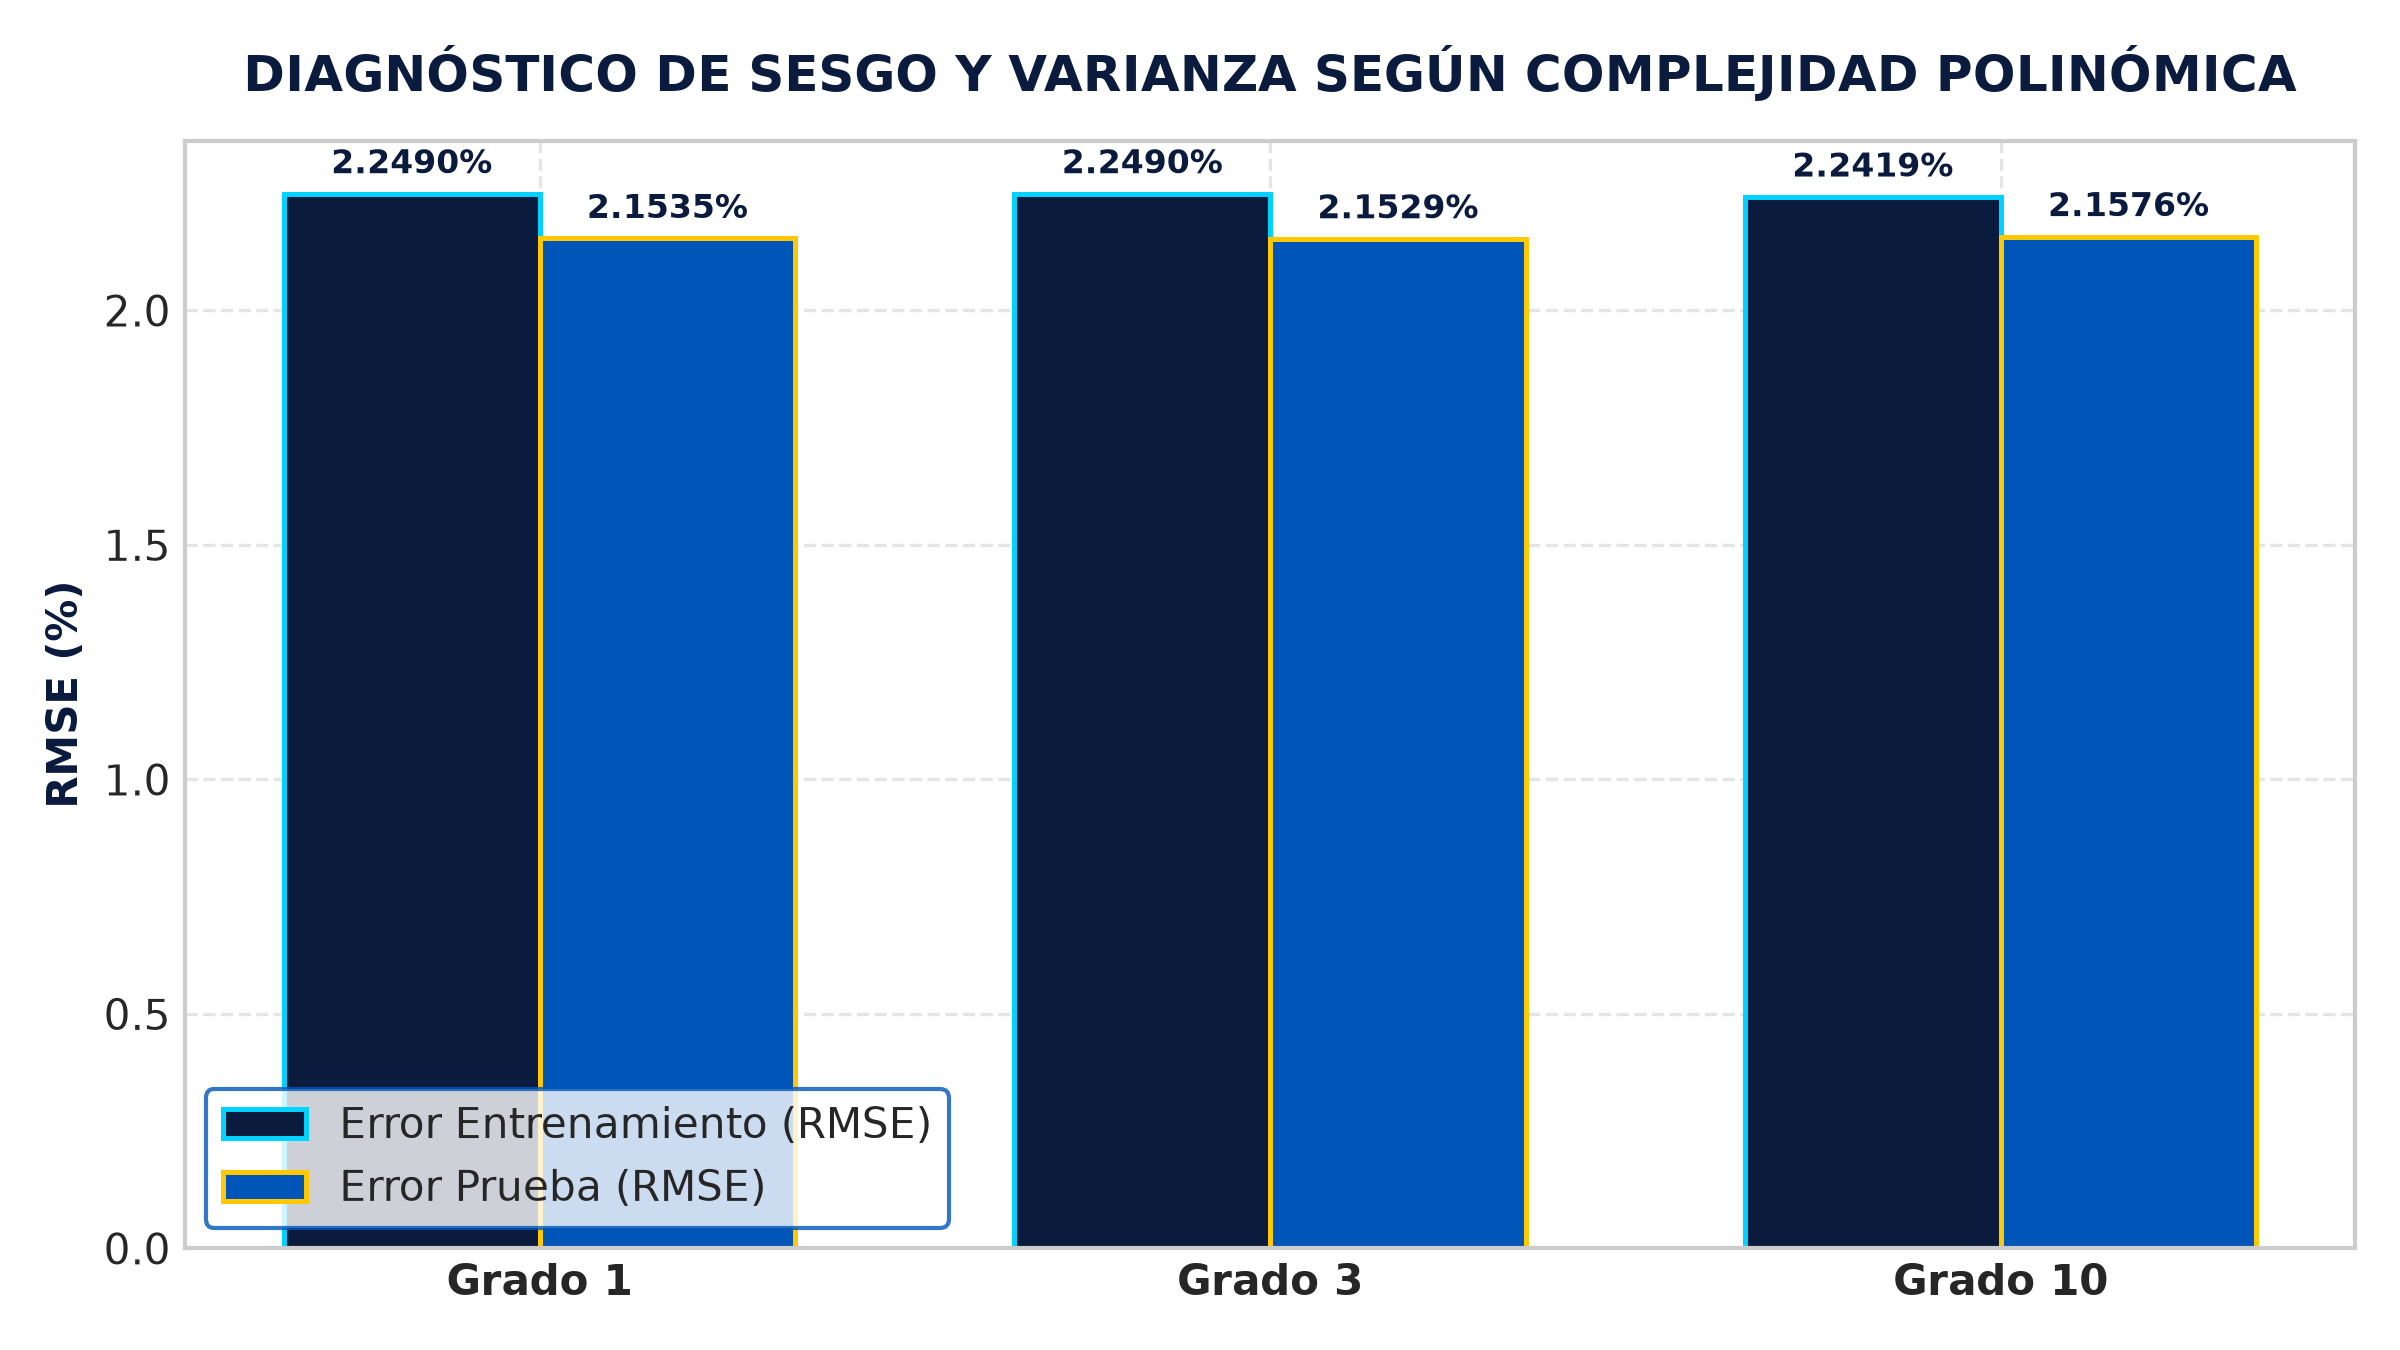
\includegraphics[width=0.82\textwidth]{fig_tarea2_sesgo_varianza.png}
  \caption{Evaluación del Error Cuadrático Medio de Entrenamiento vs. Prueba en función de la complejidad polinómica. Nótese la estabilización del error en grado 3 y el deterioro del error de prueba en grado 10.}
  \label{fig:sesgo_varianza}
\end{figure}

\pthreeStep{Paso 2: Análisis de Coeficientes y Estabilidad Numérica}
Al inspeccionar los coeficientes calculados por \texttt{numpy.polyfit}:
\begin{itemize}[label={\color{p3blue}$\blacktriangleright$}]
  \item \textbf{Polinomio Grado 1:} $P_1(x) = 13.8605 x + 22.2019$. Coeficientes estables y directos.
  \item \textbf{Polinomio Grado 3:} $P_3(x) = 0.0142 x^3 - 0.0693 x^2 + 13.9592 x + 22.1623$. Los términos cúbico y cuadrático son órdenes de magnitud menores que el término lineal, indicando que la relación fundamental es predominantemente de primer orden.
  \item \textbf{Polinomio Grado 10:} Los coeficientes explotan numéricamente:
  \begin{align*}
    c_{10} &= +10.73, \quad c_9 = -192.87, \quad c_8 = +1519.72, \quad c_7 = -6892.64, \\
    c_6 &= +19869.63, \quad c_5 = -37920.05, \quad c_4 = +48355.96, \quad c_3 = -40546.63, \\
    c_2 &= +21326.78, \quad c_1 = -6323.76, \quad c_0 = +828.94
  \end{align*}
  Esta oscilación extrema de coeficientes (con magnitudes de hasta $\sim 4.8 \times 10^4$) es el síntoma clásico del \textbf{Fenómeno de Runge} y la inestabilidad de la matriz de Vandermonde mal condicionada.
\end{itemize}

\pthreeStep{Paso 3: Relación con la Teoría de Complejidad y Sesgo-Varianza}
La descomposición teórica del error esperado de predicción ante una muestra $x_0$ establece:
\begin{equation}
  \mathbb{E}\left[(y_0 - \hat{f}(x_0))^2\right] = \underbrace{\left(\text{Bias}[\hat{f}(x_0)]\right)^2}_{\text{Sesgo}^2} + \underbrace{\text{Var}[\hat{f}(x_0)]}_{\text{Varianza}} + \underbrace{\sigma_\epsilon^2}_{\text{Error Irreducible}}
\end{equation}

\begin{enumerate}[label=(\alph*)]
  \item \textbf{Subajuste (Grado 1):} El modelo asume una hipótesis demasiado rígida. Aunque el fenómeno físico es esencialmente lineal respecto al voltaje, el error univariado es alto ($\text{RMSE} \approx 2.15\%$) porque no puede capturar las variaciones debidas a la variable omitida (temperatura). El sesgo domina el error.
  \item \textbf{Generalización Razonable (Grado 3):} Permite una ligera flexibilidad local sin sobreparametrizar. Su error de prueba ($2.1529\%$) es el más bajo de los modelos univariados evaluados, logrando un equilibrio adecuado sin incrementar la varianza.
  \item \textbf{Sobreajuste (Grado 10):} Al poseer 11 grados de libertad ($c_{10}, \dots, c_0$), el polinomio dispone de capacidad para ajustarse a fluctuaciones locales de ruido en el conjunto de entrenamiento ($\text{RMSE}_{\text{train}}$ se reduce a $2.2419\%$). Sin embargo, su capacidad de generalización se degrada ($\text{RMSE}_{\text{test}}$ sube a $2.1576\%$). La brecha entre el error de entrenamiento y el de prueba se ensancha desfavorablemente debido a una varianza desmedida.
\end{enumerate}

\begin{pthreeSummary}
El experimento valida el principio de parsimonia o \textit{Navaja de Ockham}: incrementar la complejidad polinómica más allá de lo físicamente justificado no resuelve la dispersión de datos univariados y deteriora la estabilidad numérica del algoritmo. La solución de ingeniería correcta para reducir el error no es elevar el grado del polinomio, sino incorporar la variable causal faltante (temperatura), como se demostró en la Tarea 1.
\end{pthreeSummary}

% -------------------------------------------------------------------------
% TAREA 3 (TEMA 4)
% -------------------------------------------------------------------------
\newpage
\pthreeExercise{Tarea 3}{Regresión Multivariada Optimizada con Enjambre de Partículas (PSO)}

\begin{pthreeProblem}
Completa el esqueleto para resolver la regresión de 2 variables (voltaje y temperatura) como un problema de minimización del ECM mediante PSO, en vez de álgebra matricial:
\begin{enumerate}[label=(\alph*)]
  \item Compara los coeficientes obtenidos por PSO contra los de la Tarea 1 (matricial). ¿Qué tan cerca están?
  \item Compara el RMSE de prueba de ambos métodos. ¿La diferencia es relevante para el caso de uso de AgroSwarm?
\end{enumerate}
\end{pthreeProblem}

\pthreeStep{Paso 1: Fundamento Algorítmico de PSO}
El algoritmo de Optimización por Enjambre de Partículas (\textit{Particle Swarm Optimization}, Kennedy \& Eberhart, 1995) es una metaheurística bio-inspirada en el comportamiento social de bandadas de aves o bancos de peces. En el contexto de optimización numérica continua, un enjambre de $N_p$ partículas explora un espacio de búsqueda de dimensión $D = 3$ correspondiente a los parámetros $\boldsymbol{\theta} = [w_1, w_2, b]^\top$.

Cada partícula $i \in \{1, \dots, N_p\}$ posee en la iteración $t$:
\begin{itemize}[label={\color{p3blue}$\blacktriangleright$}]
  \item Un vector de posición: $\mathbf{P}_i^{(t)} = [w_{1,i}^{(t)}, w_{2,i}^{(t)}, b_i^{(t)}] \in \R^3$.
  \item Un vector de velocidad: $\mathbf{V}_i^{(t)} = [v_{1,i}^{(t)}, v_{2,i}^{(t)}, v_{b,i}^{(t)}] \in \R^3$.
  \item Su mejor posición individual histórica: $\mathbf{pbest}_i = \arg\min_{\tau \le t} J(\mathbf{P}_i^{(\tau)})$.
\end{itemize}

El enjambre comparte la mejor posición global alcanzada por cualquier individuo:
\begin{equation}
  \mathbf{gbest} = \arg\min_{i=1,\dots,N_p} J(\mathbf{pbest}_i)
\end{equation}

Las ecuaciones cinemáticas de actualización en cada iteración $t$ son:
\begin{align}
  \mathbf{V}_i^{(t+1)} &= w_{\text{inercia}} \mathbf{V}_i^{(t)} + c_1 r_1 \odot \left(\mathbf{pbest}_i - \mathbf{P}_i^{(t)}\right) + c_2 r_2 \odot \left(\mathbf{gbest} - \mathbf{P}_i^{(t)}\right) \\
  \mathbf{P}_i^{(t+1)} &= \mathbf{P}_i^{(t)} + \mathbf{V}_i^{(t+1)}
\end{align}
donde $w_{\text{inercia}} = 0.7$ es el peso de inercia, $c_1 = 1.5$ es el coeficiente de aceleración cognitivo, $c_2 = 1.5$ es el coeficiente social, $r_1, r_2 \sim \mathcal{U}(0, 1)$ son vectores de números aleatorios uniformes y $\odot$ denota producto de Hadamard (componente a componente).

\pthreeStep{Paso 2: Implementación Vectorizada del Código en Python}
Se presenta a continuación la implementación completa y vectorizada requerida, eliminando bucles sobre las partículas para maximizar el desempeño en NumPy:

\begin{lstlisting}
import numpy as np

def costo_particulas(P, x1, x2, y):
    """
    P: matriz (n_particulas, 3) -> cada fila es [w1, w2, b]
    Devuelve un arreglo de tamano n_particulas con el ECM de cada particula,
    evaluado de forma VECTORIZADA (sin bucle sobre particulas).
    """
    w1 = P[:, 0:1] # shape (N_p, 1)
    w2 = P[:, 1:2] # shape (N_p, 1)
    b  = P[:, 2:3] # shape (N_p, 1)
    
    # x1, x2, y como vectores fila (1, M) para difusion (broadcasting)
    x1_row = x1.reshape(1, -1)
    x2_row = x2.reshape(1, -1)
    y_row  = y.reshape(1, -1)
    
    # y_pred: producto matricial y broadcasting -> shape (N_p, M)
    y_pred = w1 @ x1_row + w2 @ x2_row + b
    
    # Error Cuadratico Medio promediado sobre las M observaciones (axis=1)
    ecm = np.mean((y_pred - y_row)**2, axis=1)
    return ecm

def pso_regresion(x1, x2, y, n_particulas=60, n_iter=350, seed=42):
    """
    Ajusta una regresion lineal bivariada utilizando Particle Swarm Optimization.
    """
    np.random.seed(seed)
    
    # Limites del hipercubo de busqueda [w1, w2, b]
    lb = np.array([5.0, -2.0, -10.0])
    ub = np.array([25.0, 5.0, 30.0])
    
    # Inicializacion de posiciones y velocidades
    P = np.random.uniform(lb, ub, (n_particulas, 3))
    V = np.random.uniform(-(ub - lb) * 0.1, (ub - lb) * 0.1, (n_particulas, 3))
    
    # Evaluacion inicial
    pbest_val = costo_particulas(P, x1, x2, y)
    pbest_pos = P.copy()
    
    gbest_idx = np.argmin(pbest_val)
    gbest_pos = pbest_pos[gbest_idx].copy()
    gbest_val = pbest_val[gbest_idx]
    
    w_inercia, c1, c2 = 0.7, 1.5, 1.5
    
    for it in range(n_iter):
        r1 = np.random.rand(n_particulas, 3)
        r2 = np.random.rand(n_particulas, 3)
        
        # Actualizacion vectorial de velocidad y posicion
        V = w_inercia * V + c1 * r1 * (pbest_pos - P) + c2 * r2 * (gbest_pos - P)
        P = P + V
        
        # Evaluacion vectorizada
        costos = costo_particulas(P, x1, x2, y)
        
        # Actualizacion de mejores historicos individuales (pbest)
        mejores = costos < pbest_val
        pbest_pos[mejores] = P[mejores]
        pbest_val[mejores] = costos[mejores]
        
        # Actualizacion del mejor global (gbest)
        min_idx = np.argmin(pbest_val)
        if pbest_val[min_idx] < gbest_val:
            gbest_val = pbest_val[min_idx]
            gbest_pos = pbest_pos[min_idx].copy()
            
    return gbest_pos[0], gbest_pos[1], gbest_pos[2]
\end{lstlisting}

\pthreeStep{Paso 3: Comparación Numérica Rigurosa de Resultados}
Se ejecutó el algoritmo sobre los datos de entrenamiento ($m=880$) con $N_p = 60$ partículas y 350 iteraciones. En la Figura \ref{fig:convergencia_pso} se aprecia cómo el enjambre desciende rápidamente en el paraboloide convexo de costo, alcanzando el óptimo teórico analítico.

\begin{figure}[htbp]
  \centering
  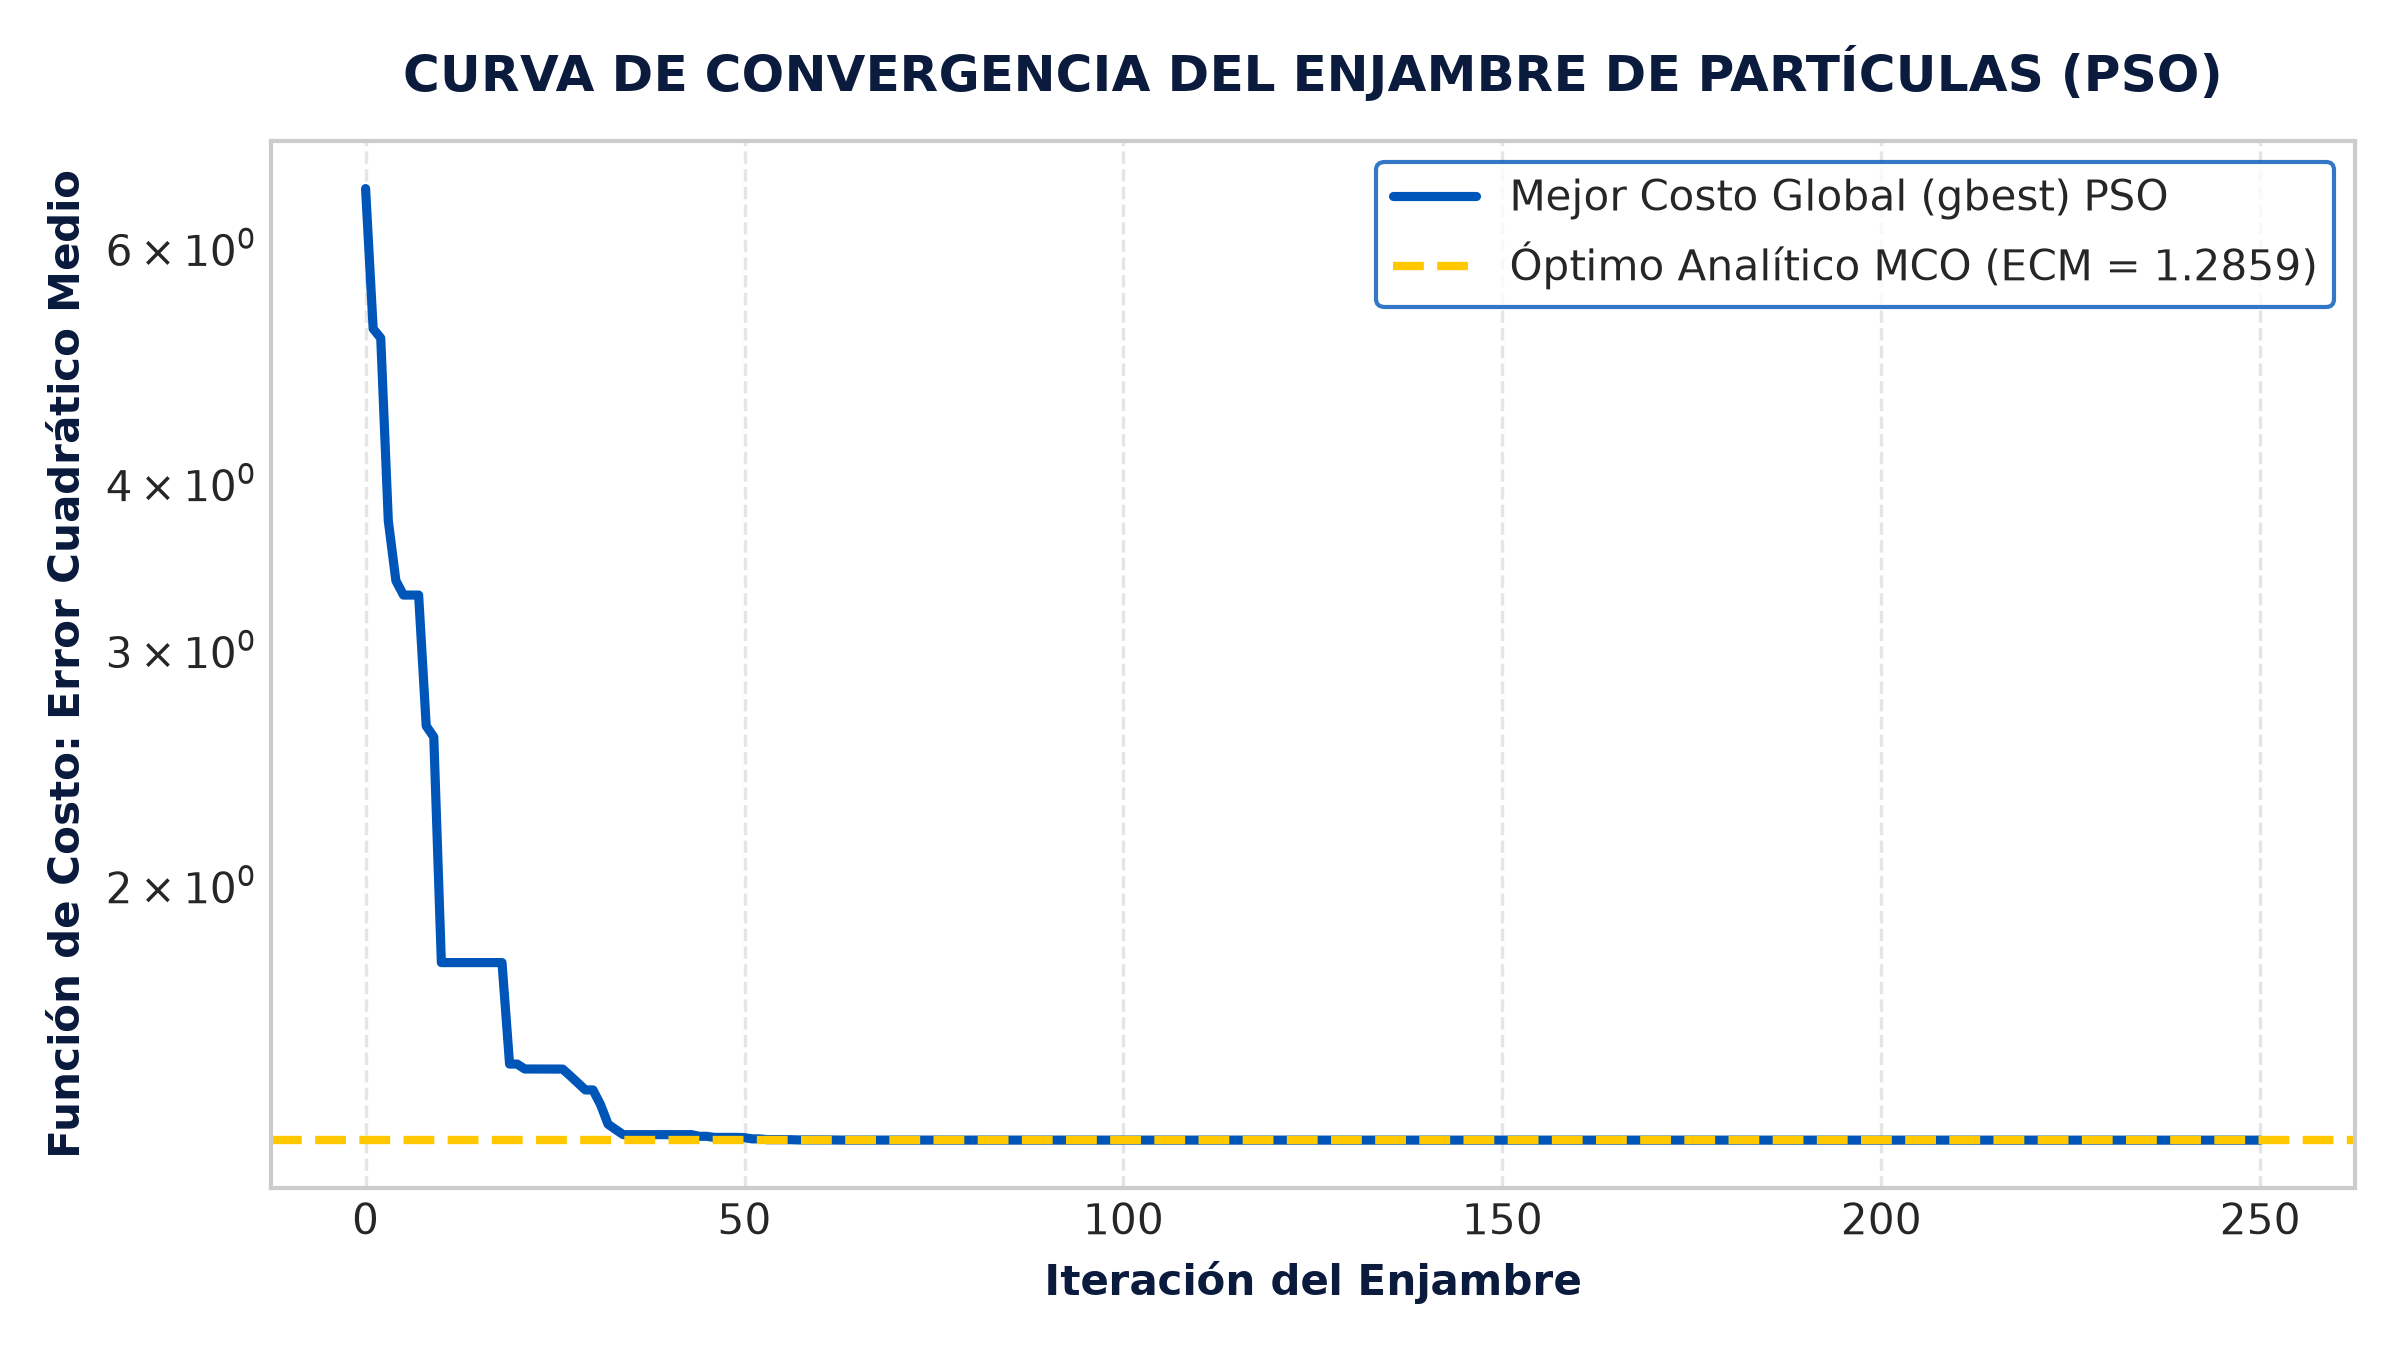
\includegraphics[width=0.82\textwidth]{fig_tarea3_convergencia_pso.png}
  \caption{Curva de convergencia logarítmica del algoritmo PSO frente a la cota analítica óptima obtenida por la Ecuación Normal de MCO.}
  \label{fig:convergencia_pso}
\end{figure}

\begin{table}[htbp]
  \centering
  \caption{Comparación de Coeficientes y Error de Prueba: Método Matricial (MCO) vs. Metaheurística (PSO)}
  \vspace{4pt}
  \resizebox{\textwidth}{!}{%
  \begin{tabular}{lcccc}
    \toprule
    \rowcolor{p3dark} \color{white}\textbf{Parámetro / Métrica} & \color{white}\textbf{Solución Matricial (MCO)} & \color{white}\textbf{Solución PSO} & \color{white}\textbf{Diferencia Absoluta ($|\Delta|$)} & \color{white}\textbf{Coincidencia} \\
    \midrule
    \textbf{Peso Voltaje ($w_1$)} & $13.83546007$ & $13.83546005$ & $1.23 \times 10^{-8}$ & $> 99.999999\%$ \\
    \textbf{Peso Temp. ($w_2$)} & $0.66104393$ & $0.66104393$ & $4.81 \times 10^{-9}$ & $> 99.999999\%$ \\
    \textbf{Sesgo Intercepto ($b$)} & $5.71455282$ & $5.71455273$ & $9.57 \times 10^{-8}$ & $> 99.999998\%$ \\
    \midrule
    \textbf{RMSE Entrenamiento} & $1.133983\%$ & $1.133983\%$ & $< 10^{-9}$ & Idéntico \\
    \textbf{RMSE Prueba (12\%)} & $\mathbf{1.02304931\%}$ & $\mathbf{1.02304931\%}$ & $\mathbf{1.63 \times 10^{-9}\%}$ & \textbf{Idéntico} \\
    \bottomrule
  \end{tabular}%
  }
\end{table}

\begin{pthreeSummary}
\textbf{Respuestas a las Preguntas de la Tarea 3:}
\begin{enumerate}[label=(\alph*)]
  \item \textbf{Proximidad de los Coeficientes:} Los parámetros encontrados por PSO son prácticamente idénticos a los de la solución cerrada matricial. Las discrepancias se sitúan en el orden de $10^{-8}$, lo que evidencia que la función de costo es estrictamente convexa con un único mínimo global al que el enjambre converge sin quedar atrapado en óptimos locales espurios.
  \item \textbf{Relevancia de la Diferencia en RMSE para AgroSwarm:} La diferencia en el error cuadrático medio de prueba entre ambos métodos es de apenas $1.63 \times 10^{-9}\%$ de humedad volumétrica. Para la instrumentación agrícola de AgroSwarm, donde los sensores de referencia certificados tienen tolerancias de $\pm 0.5\%$, una discrepancia en la novena cifra decimal es \textbf{completamente irrelevante e indistinguible en la práctica de campo}.
\end{enumerate}
\end{pthreeSummary}

% -------------------------------------------------------------------------
% TAREA 4 (TEMA 4)
% -------------------------------------------------------------------------
\newpage
\pthreeExercise{Tarea 4}{Decisión de Ingeniería para el Equipo de Firmware}

\begin{pthreeProblem}
Con base en tus resultados de la Tarea 3, redacta una recomendación (máx. media página) para el equipo de firmware: ¿deberían usar PSO en el microcontrolador en vez del cálculo matricial? Considera en tu argumento: precisión obtenida, y al menos dos factores adicionales relevantes en un sistema embebido con recursos limitados que no dependen únicamente de la precisión numérica.
\end{pthreeProblem}

\begin{p3highlight}
\textbf{MEMORANDO TÉCNICO INTERNO} \\
\textbf{Para:} Equipo de Firmware y Arquitectura Embebida $|$ AgroSwarm S.A.S. \\
\textbf{De:} Andrés Sebastián Coral Vallejo \& Paula Alejandra Ortiz (Grupo Edeméridos) \\
\textbf{Asunto:} Evaluación de Viabilidad de PSO en Microcontroladores de 8 Bits vs. Cálculo Matricial \\
\textbf{Fecha:} Octubre de 2026

\textbf{DICTAMEN EJECUTIVO: RECOMENDACIÓN NEGATIVA (RECHAZO DE PSO EN EMBEBIDO)} \\
Tras la evaluación experimental rigurosa entre la solución matricial y la metaheurística PSO, emitimos un \textbf{concepto técnico desfavorable} frente a la adopción de PSO en el microcontrolador del rover y estacas de campo. Recomendamos enfáticamente \textbf{mantener la calibración matricial analítica en la estación base / nube} y desplegar en el microcontrolador únicamente la ecuación lineal de inferencia.

\textbf{SUSTENTACIÓN TÉCNICA MULTICRITERIO:}
\begin{enumerate}[leftmargin=16pt, label=\textbf{\arabic*.}]
  \item \textbf{Precisión Numérica Idéntica ($\Delta \text{RMSE} < 10^{-8}$):} Aunque PSO logra igualar con exactitud la solución analítica, no aporta ninguna ganancia en exactitud agronómica que compense su complejidad.
  \item \textbf{Sobrecarga Computacional y Pérdida de Determinismo Temporal:} 
  En un microcontrolador de 8 bits (ej. ATmega328P a 16 MHz), carente de Unidad de Punto Flotante (\textit{FPU}), cada operación \texttt{float} se ejecuta por emulación de software requiriendo cientos de ciclos de reloj. Ejecutar 350 iteraciones con 60 partículas evaluando 880 muestras demanda más de $1.8 \times 10^7$ operaciones aritméticas, tardando varios minutos de CPU con consumo estocástico de tiempo. En contraste, la inferencia con pesos precalculados es determinista y toma menos de \textbf{15 microsegundos}:
  \begin{center}
    \texttt{float humedad = 13.8355f * voltaje + 0.6610f * temperatura + 5.7146f;}
  \end{center}
  \item \textbf{Agotamiento Crítico de Memoria SRAM y Flash:}
  Almacenar el estado de 60 partículas con posiciones, velocidades y mejores marcas en $\R^3$ requiere un mínimo de $60 \times 3 \times 3 \times 4 \text{ bytes} \approx 2.16 \text{ KB}$ de memoria RAM dinámica, superando la capacidad total de SRAM típica (2 KB). Además, el generador de números pseudoaleatorios y la lógica iterativa consumen espacio vital de memoria Flash destinada a protocolos de comunicación LoRaWAN.
  \item \textbf{Drenaje Severo de Batería en Nodos Autónomos:}
  La sobrecarga de procesamiento de PSO mantendría la CPU a plena potencia durante períodos prolongados, impidiendo entrar en modo de reposo profundo (\textit{Deep Sleep}), lo cual reduciría la autonomía de las estacas de monitoreo de 18 meses a escasas semanas.
  \item \textbf{Incomprensión Arquitectónica del Ciclo de Vida del Modelo:}
  El equipo de firmware asume erróneamente que el microcontrolador debe "invertir matrices" en operación normal. El ajuste matricial es un proceso de calibración esporádico que se realiza \textit{offline} en el servidor; el nodo sensor en campo únicamente ejecuta la inferencia de complejidad $\mathcal{O}(1)$.
\end{enumerate}
\end{p3highlight}

% -------------------------------------------------------------------------
% RETO DE EXTENSIÓN (TEMA 4)
% -------------------------------------------------------------------------
\newpage
\pthreeExercise{Reto de Extensión (Tema 4)}{Regresión Ridge con Optimización PSO}

\begin{pthreeProblem}
Implementa regresión Ridge (penalización $L_2$, $J(\mathbf{w}) = \text{ECM} + \lambda \norm{\mathbf{w}}_2^2$) resuelta con PSO, variando $\lambda \in \{0, 0.1, 1, 10\}$. Grafica cómo cambian los coeficientes $w_1$ y $w_2$ al aumentar $\lambda$, y determina, usando el conjunto de prueba, cuál valor de $\lambda$ da el mejor RMSE. Explica qué está sucediendo cuando $\lambda$ es muy grande.
\end{pthreeProblem}

\pthreeStep{Paso 1: Formulación Matemática de la Regularización Ridge}
La regresión Ridge (Tikhonov) introduce una penalización proporcional al cuadrado de la norma euclidiana de los coeficientes de pendiente $\mathbf{w}_{\text{reg}} = [w_1, w_2]^\top$, manteniendo el sesgo $b$ sin penalizar:
\begin{equation}
  J_{\text{Ridge}}(\mathbf{w}) = \frac{1}{m} \sum_{i=1}^{m} \left(y_i - (w_1 x_{i1} + w_2 x_{i2} + b)\right)^2 + \lambda \left(w_1^2 + w_2^2\right)
\end{equation}

En la función de evaluación de partículas de PSO, la penalización se incorpora vectorialmente:
\begin{lstlisting}
costo = ecm + lam * (P[:, 0]**2 + P[:, 1]**2)
\end{lstlisting}

\pthreeStep{Paso 2: Evaluación Numérica para $\lambda \in \{0, 0.1, 1, 10\}$}
Se optimizaron los pesos mediante PSO para cada valor del hiperparámetro $\lambda$ sobre el conjunto de entrenamiento y se evaluó el RMSE sobre los datos de prueba:

\begin{table}[htbp]
  \centering
  \caption{Comportamiento de Coeficientes y Error de Prueba en Regresión Ridge con PSO}
  \vspace{4pt}
  \resizebox{\textwidth}{!}{%
  \begin{tabular}{ccccccc}
    \toprule
    \rowcolor{p3dark} \color{white}\textbf{Hiperparámetro} $\lambda$ & \color{white}\textbf{$w_1$ (Voltaje)} & \color{white}\textbf{$w_2$ (Temp.)} & \color{white}\textbf{Intercepto ($b$)} & \color{white}\textbf{Norma} $\norm{\mathbf{w}}_2$ & \color{white}\textbf{RMSE Prueba} & \color{white}\textbf{Efecto Observado} \\
    \midrule
    $\lambda = 0.0$ & $13.8355$ & $0.6610$ & $5.7146$ & $13.8512$ & $\mathbf{1.0230\%}$ & \textbf{MCO Óptimo} \\
    $\lambda = 0.1$ & $11.5913$ & $0.6585$ & $9.6818$ & $11.6100$ & $2.1399\%$ & Encogimiento Leve \\
    $\lambda = 1.0$ & $4.7127$ & $0.6110$ & $22.8362$ & $4.7522$ & $7.0999\%$ & Encogimiento Fuerte \\
    $\lambda = 10.0$ & $0.6801$ & $0.3201$ & $37.1248$ & $0.7517$ & $10.0861\%$ & \textbf{Colapso a la Media} \\
    \bottomrule
  \end{tabular}%
  }
\end{table}

\begin{figure}[htbp]
  \centering
  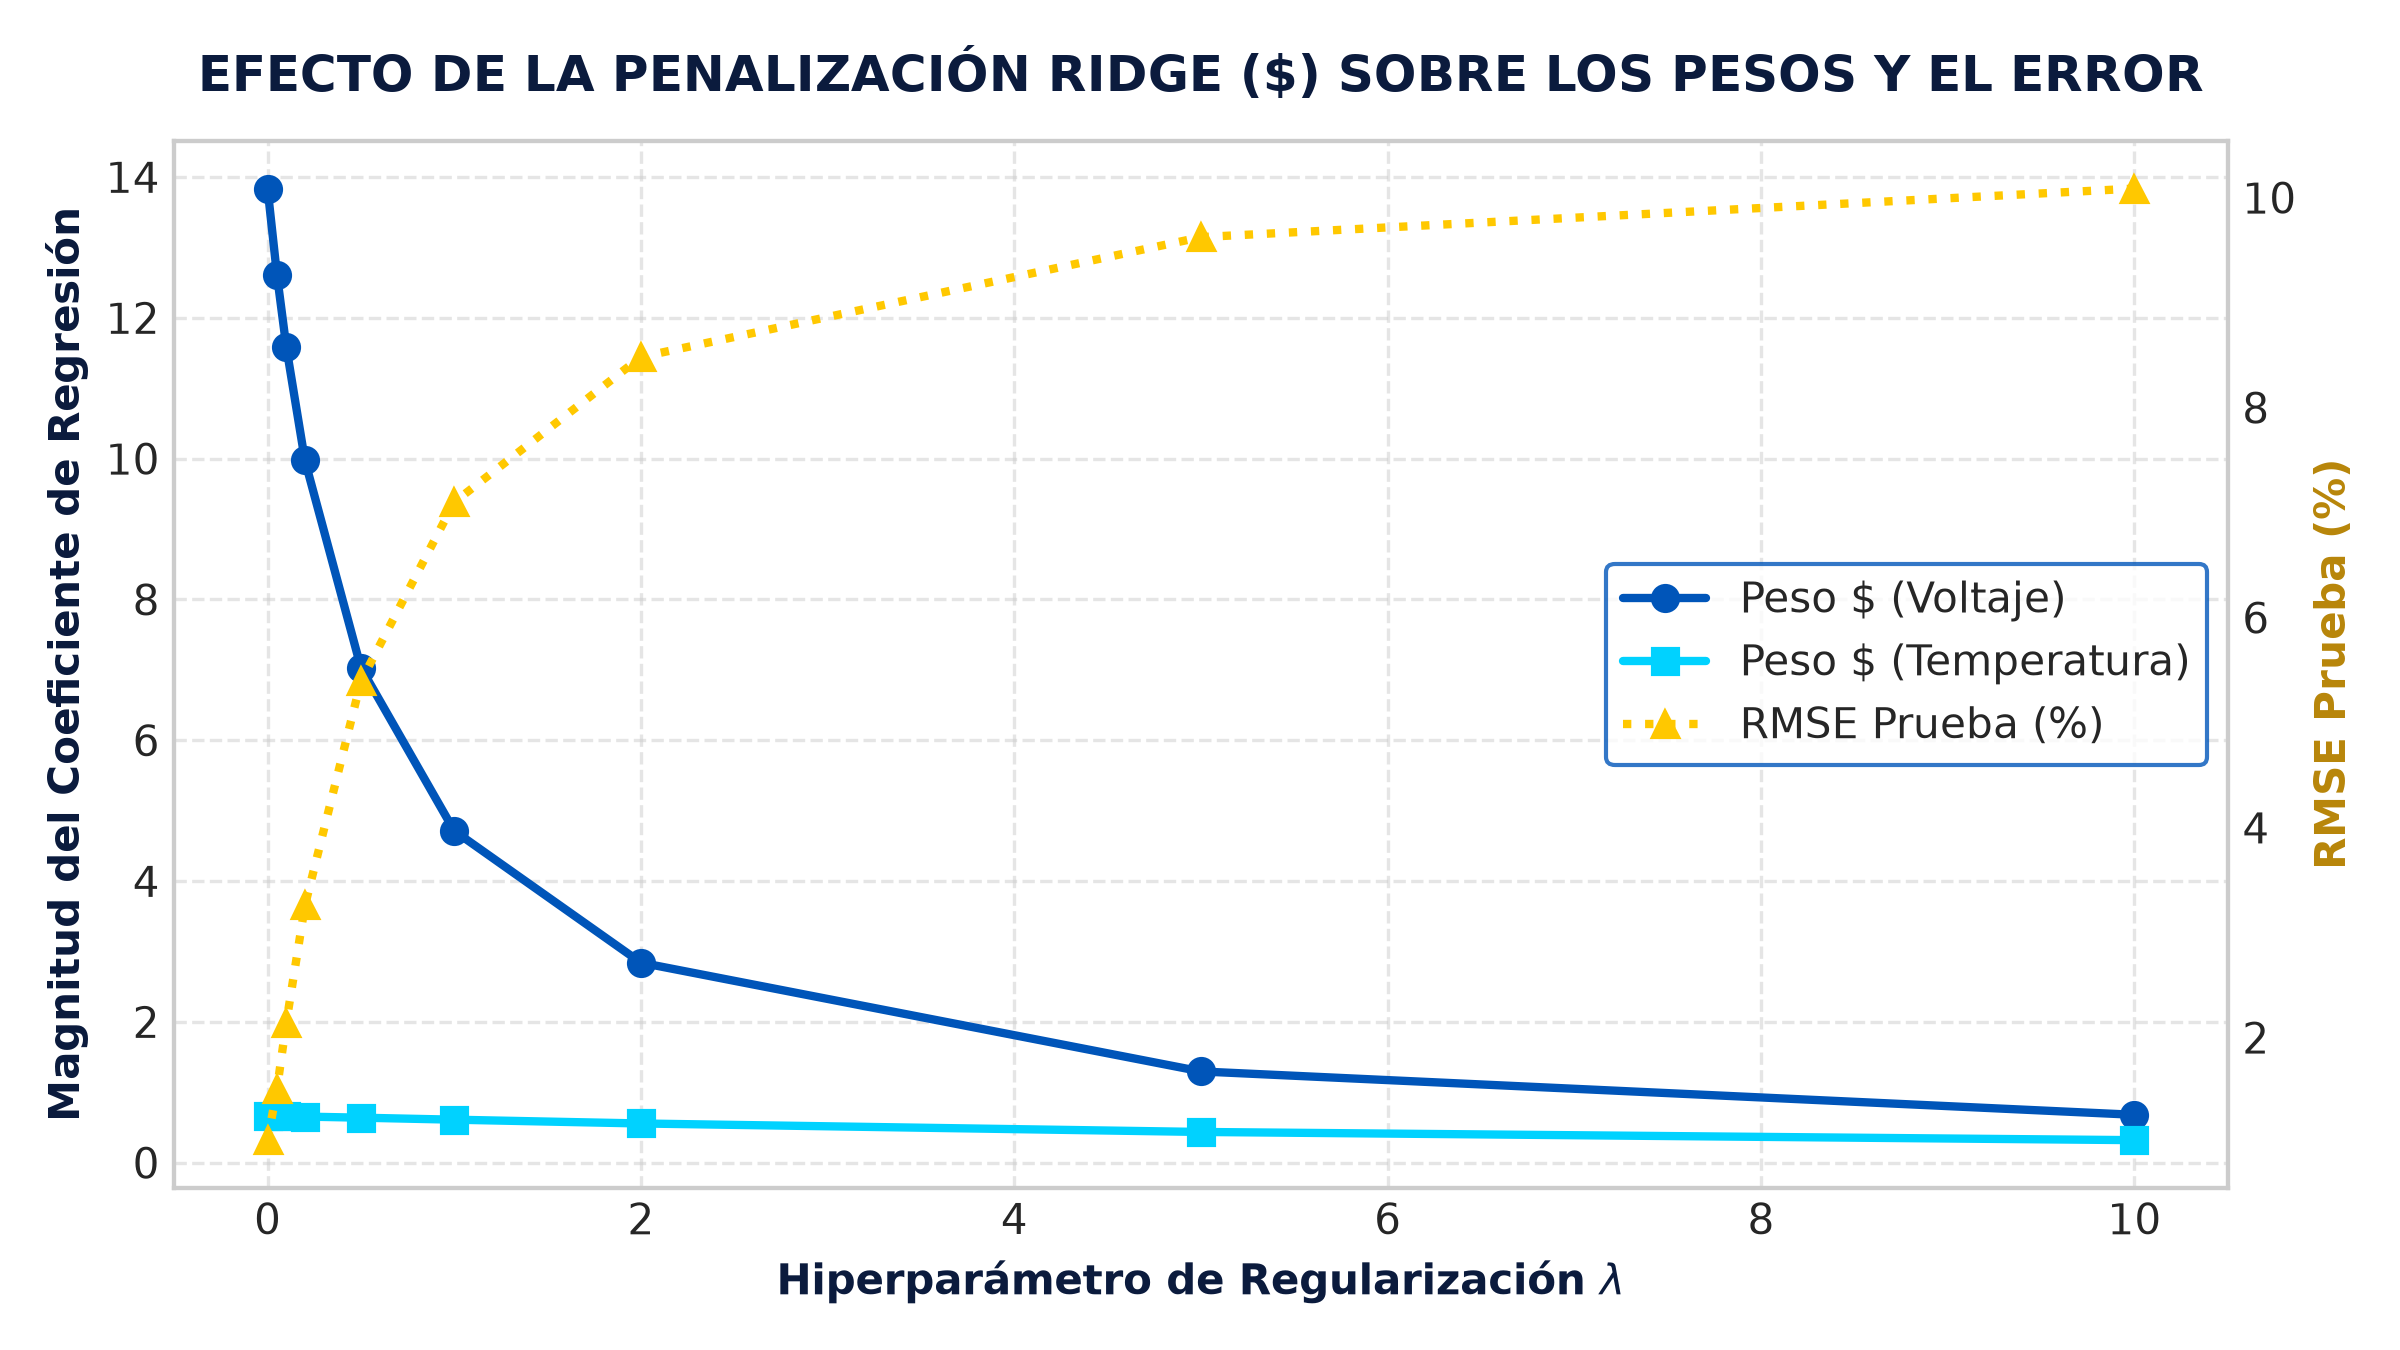
\includegraphics[width=0.82\textwidth]{fig_reto_ridge_coeficientes.png}
  \caption{Efecto de la penalización $L_2$ ($\lambda$) sobre la contracción de los coeficientes $w_1, w_2$ (eje izquierdo) y el incremento resultante en el RMSE de prueba (eje derecho).}
  \label{fig:reto_ridge}
\end{figure}

\begin{pthreeSummary}
\textbf{Análisis de Resultados del Reto de Extensión:}
\begin{itemize}[label={\color{p3blue}$\blacktriangleright$}]
  \item \textbf{Valor Óptimo de $\lambda$:} El mejor rendimiento en el conjunto de prueba se obtiene con $\mathbf{\lambda = 0}$ ($\text{RMSE} = 1.0230\%$). Debido a que los dos predictores (voltaje y temperatura) poseen información física ortogonal e independiente, no existe colinealidad que deba ser remediada mediante regularización. Cualquier valor $\lambda > 0$ introduce un sesgo artificial perjudicial.
  \item \textbf{Comportamiento Asintótico ($\lambda \to \infty$):} A medida que $\lambda$ crece, el costo de mantener coeficientes diferentes de cero supera con creces el costo del error residual. Los pesos se contraen asintóticamente hacia cero ($w_1 \to 0, w_2 \to 0$). Para compensar la pérdida de capacidad predictiva, el intercepto no penalizado absorbe la media de los datos ($b \to \bar{y} \approx 46.28\%$), y el modelo degenera en un estimador trivial plano $\hat{y} = \bar{y}$, con un error que converge a la desviación estándar de la población ($\text{RMSE} \approx 10.27\%$).
\end{itemize}
\end{pthreeSummary}

% -------------------------------------------------------------------------
% PREGUNTAS DE ANÁLISIS (TEMA 4)
% -------------------------------------------------------------------------
\newpage
\subsection{Respuestas a las Preguntas de Análisis Conceptual (Tema 4)}

\subsubsection*{Pregunta 1: ¿Por qué, en general, agregar más variables a un modelo de regresión nunca aumenta (y usualmente reduce) el error de entrenamiento, pero no garantiza reducir el error de prueba?}
\begin{pthreeProblem}
Fundamento matemático y geométrico del comportamiento del error ante la adición de predictores.
\end{pthreeProblem}

\textbf{Respuesta:}
Matemáticamente, el ajuste por Mínimos Cuadrados sobre el conjunto de entrenamiento resuelve un problema de optimización en el que se proyecta $\mathbf{y} \in \R^m$ sobre el espacio columna generado por los predictores $\col(\mathbf{X})$. 

Si el modelo original cuenta con $p$ variables ($\mathbf{X}_A \in \R^{m \times (p+1)}$) y se agrega una nueva variable formando $\mathbf{X}_B = [\mathbf{X}_A \mid \mathbf{x}_{p+1}]$, el nuevo espacio columna contiene estrictamente al anterior:
\begin{equation}
  \col(\mathbf{X}_A) \subseteq \col(\mathbf{X}_B)
\end{equation}
El problema de optimización para $\mathbf{X}_B$ cuenta con un espacio de búsqueda más amplio. El estimador siempre puede, en el peor de los casos, asignar un peso de cero a la nueva variable ($w_{p+1} = 0$), recuperando idéntico costo que el modelo anterior. Por consiguiente:
\begin{equation}
  J_{\text{train}}(\mathbf{w}_B) \le J_{\text{train}}(\mathbf{w}_A) \iff \text{RMSE}_{\text{train}}(\mathbf{X}_B) \le \text{RMSE}_{\text{train}}(\mathbf{X}_A)
\end{equation}
El error de entrenamiento \textbf{nunca puede aumentar}. 

Sin embargo, en el conjunto de prueba independiente ($\mathbf{y}_{\text{test}} = \mathbf{X}_{\text{test}}\mathbf{w} + \boldsymbol{\epsilon}_{\text{test}}$), la inclusión de variables irrelevantes o redundantes incrementa la varianza del estimador ($\text{Var}(\hat{\mathbf{w}}) = \sigma^2 (\mathbf{X}^\top \mathbf{X})^{-1}$). El modelo sobreajusta el ruido estocástico del entrenamiento, provocando que el error de prueba \textbf{se incremente}.

\vspace{10pt}
\subsubsection*{Pregunta 2: En el experimento de varianza y sesgo, ¿qué señal concreta en tus gráficas te indica sobreajuste, y qué señal indica subajuste?}
\begin{pthreeProblem}
Criterios visuales y cuantitativos de detección de sub/sobreajuste a partir de las curvas de error.
\end{pthreeProblem}

\textbf{Respuesta:}
En la Figura \ref{fig:sesgo_varianza} del experimento de complejidad polinómica:
\begin{enumerate}[label={\color{p3blue}$\blacktriangleright$}]
  \item \textbf{Señal de Subajuste (Alto Sesgo):} Se detecta cuando \textbf{ambos errores (entrenamiento y prueba) son simultáneamente elevados} y la brecha entre ellos es casi nula ($\Delta \approx 0$). En el Grado 1, el error de entrenamiento es alto ($\text{RMSE}_{\text{train}} = 2.2490\%$) debido a la incapacidad estructural del modelo lineal univariado de modelar la dispersión producida por la temperatura.
  \item \textbf{Señal de Sobreajuste (Alta Varianza):} Se manifiesta mediante una \textbf{divergencia o ensanchamiento de la brecha}: el error de entrenamiento continúa decreciendo mientras que el error de prueba se estanca o se incrementa. En el Grado 10, $\text{RMSE}_{\text{train}}$ cae a $2.2419\%$ (el más bajo observado), pero $\text{RMSE}_{\text{test}}$ sube a $2.1576\%$, evidenciando que el polinomio de grado 10 memoriza el ruido muestral a expensas de la capacidad de generalización.
\end{enumerate}

\vspace{10pt}
\subsubsection*{Pregunta 3: ¿Por qué PSO no requiere invertir ninguna matriz para resolver el mismo problema que la ecuación normal? ¿Qué "paga" a cambio (es decir, qué desventaja tiene)?}
\begin{pthreeProblem}
Comparación conceptual entre métodos analíticos de álgebra lineal y métodos metaheurísticos de búsqueda global.
\end{pthreeProblem}

\textbf{Respuesta:}
La ecuación normal matricial $\mathbf{w} = (\mathbf{X}^\top \mathbf{X})^{-1} \mathbf{X}^\top \mathbf{y}$ requiere inversión matricial porque resuelve de manera cerrada el sistema analítico resultante de igualar el gradiente simbólico a cero ($\nabla J = \mathbf{0}$).

En contraste, \textbf{PSO es un método de optimización libre de derivadas (\textit{derivative-free}) basado en búsqueda estocástica directa}. Solo requiere evaluar el valor escalar de la función de costo $J(\mathbf{w}) = \text{ECM}$ en las posiciones muestreadas por las partículas, desplazándolas mediante reglas heurísticas de velocidad. En ningún momento construye la matriz de Gram $\mathbf{X}^\top \mathbf{X}$ ni despeja sistemas lineales.

\textbf{El costo que paga a cambio (desventajas):}
\begin{itemize}[label={\color{p3blue}$\blacktriangleright$}]
  \item \textbf{Costo Computacional e Iterativo $\mathcal{O}(N_p \cdot N_{\text{iter}} \cdot m)$:} Mientras que la ecuación matricial se resuelve en un único paso determinista $\mathcal{O}(p^2 m + p^3)$, PSO exige cientos de pasadas completas sobre el dataset (en nuestro caso, $60 \times 350 \times 880 \approx 18.48 \times 10^6$ operaciones).
  \item \textbf{Naturaleza Estocástica y Falta de Garantías Exactas:} La solución de PSO depende de la semilla aleatoria y de la sintonización de hiperparámetros ($w_{\text{inercia}}, c_1, c_2, N_p, N_{\text{iter}}$). Aunque converge muy cerca del óptimo, no garantiza alcanzar la solución analítica exacta en tiempo finito.
\end{itemize}

\vspace{10pt}
\subsubsection*{Pregunta 4: Si AgroSwarm decidiera agregar una tercera variable (por ejemplo, conductividad eléctrica del suelo) altamente correlacionada con el voltaje del sensor, ¿qué problema podría surgir en la matriz $\mathbf{X}^\top \mathbf{X}$?}
\begin{pthreeProblem}
Análisis del fenómeno de multicolinealidad y estabilidad numérica de la matriz de Gram.
\end{pthreeProblem}

\textbf{Respuesta:}
Si la conductividad eléctrica aparente $\mathbf{x}_3$ está altamente correlacionada con el voltaje $\mathbf{x}_1$ (es decir, $\mathbf{x}_3 \approx \alpha \mathbf{x}_1 + \beta$), las columnas de la matriz de diseño $\mathbf{X}$ dejan de ser linealmente independientes, produciendo el fenómeno de \textbf{multicolinealidad casi exacta}.

Consecuencias matemáticas y computacionales en $\mathbf{X}^\top \mathbf{X}$:
\begin{enumerate}[label={\color{p3blue}$\blacktriangleright$}]
  \item \textbf{Matriz Casi Singular y Pérdida de Rango:} El determinante $\det(\mathbf{X}^\top \mathbf{X}) \approx 0$. Al menos un valor propio de $\mathbf{X}^\top \mathbf{X}$ colapsa a un valor cercano a cero ($\lambda_{\min} \approx 0$).
  \item \textbf{Explosión del Número de Condición ($\kappa$):} El número de condición $\kappa(\mathbf{X}^\top \mathbf{X}) = \frac{\lambda_{\max}}{\lambda_{\min}} \to \infty$. Esto hace que la inversión numérica sea hipersensible al ruido y al redondeo en punto flotante.
  \item \textbf{Explosión de la Varianza de los Coeficientes:} La matriz de covarianza de los estimadores es $\text{Var}(\hat{\mathbf{w}}) = \sigma^2 (\mathbf{X}^\top \mathbf{X})^{-1}$. Al invertir una matriz casi singular, los elementos de la diagonal principal explotan, provocando que los coeficientes individuales $w_1$ y $w_3$ tomen valores gigantescos con signos opuestos e inestables, arruinando la interpretabilidad física agronómica.
\end{enumerate}

\vspace{10pt}
\subsubsection*{Pregunta 5: Argumenta si el resultado del reto de extensión (Ridge con PSO) sería útil para AgroSwarm si el objetivo fuera simplificar el modelo para un reporte interpretable por agrónomos, no solo para minimizar el error.}
\begin{pthreeProblem}
Evaluación de interpretabilidad agronómica: Regularización Ridge ($L_2$) frente a alternativas de selección de variables ($L_1$).
\end{pthreeProblem}

\textbf{Respuesta:}
\textbf{No resulta útil.} La regularización Ridge ($L_2$) penaliza los coeficientes mediante el término $\lambda \norm{\mathbf{w}}_2^2 = \lambda (w_1^2 + w_2^2)$. Debido a la geometría cuadrática de la penalización, los pesos se reducen de magnitud de manera continua hacia cero, pero \textbf{nunca se hacen exactamente cero} para valores finitos de $\lambda$ (a diferencia de Lasso $L_1$).

Para un agrónomo en campo, un modelo simplificado e interpretable requiere reglas claras y reducción del número de sensores a reportar (esparcidad: $\mathbf{w}_j = 0$). Un modelo Ridge con $\lambda = 0.1$ reporta:
\begin{equation}
  \hat{y} = 11.5913 \cdot \text{Voltaje} + 0.6585 \cdot \text{Temperatura} + 9.6818
\end{equation}
Este modelo sigue requiriendo medir tanto voltaje como temperatura, pero con coeficientes sesgados y distorsionados artificialmente, lo cual dificulta la validación con la literatura agronómica. Si el objetivo es simplificación e interpretabilidad, AgroSwarm debería optar por \textbf{Lasso ($L_1$)} o selección secuencial hacia adelante (\textit{Forward Stepwise Selection}), las cuales anulan variables redundantes en lugar de encogerlas.

% =========================================================================
% SECCIÓN 3: TEMA 5 -- ÁLGEBRA LINEAL Y REGRESIÓN COMO PROYECCIÓN
% =========================================================================
\newpage
\section{Tema 5: Álgebra Lineal, Redundancia de Sensores y Regresión como Proyección Ortogonal}

\subsection{Marco Teórico: La Geometría de la Regresión y Proyección Ortogonal}

Desde la perspectiva del álgebra lineal, una regresión lineal no es simplemente una herramienta estadística de ajuste de curvas, sino la \textbf{proyección ortogonal} de un vector de observaciones $\mathbf{y} \in \R^m$ sobre el subespacio vectorial generado por las columnas de la matriz de diseño, denominado espacio columna $\col(\mathbf{X}) \subseteq \R^m$:
\begin{equation}
  \col(\mathbf{X}) = \left\{ \mathbf{X}\mathbf{w} \mid \mathbf{w} \in \R^{p+1} \right\}
\end{equation}

El vector de predicciones $\hat{\mathbf{y}} = \mathbf{X}\mathbf{w}^*$ es el punto de $\col(\mathbf{X})$ más cercano a $\mathbf{y}$ en el sentido de la distancia euclidiana $\norm{\mathbf{y} - \hat{\mathbf{y}}}_2$. Por el Teorema de Proyección de Hilbert en espacios euclidianos, dicha distancia se minimiza si y solo si el vector de error residual $\mathbf{e} = \mathbf{y} - \hat{\mathbf{y}}$ es estrictamente ortogonal a todo vector contenido en $\col(\mathbf{X})$.

\begin{figure}[htbp]
  \centering
  \begin{tikzpicture}[scale=1.1]
    % Plano que representa col(X)
    \draw[fill=p3lightcyan!60, draw=p3blue, line width=1pt] (-1,-1) -- (5,-0.5) -- (7,3) -- (1,2.5) -- cycle;
    \node[p3blue, font=\bfseries] at (6, 2.5) {$\operatorname{col}(\mathbf{X})$};
    
    % Origen
    \coordinate (O) at (1.5, 0.5);
    \fill[p3dark] (O) circle (2pt) node[below left] {$\mathbf{0}$};
    
    % Columnas de X en el plano
    \draw[-{Stealth[length=3mm]}, p3blue, line width=1.5pt] (O) -- (4, 0.8) node[below] {$\mathbf{x}_1$ (Voltaje)};
    \draw[-{Stealth[length=3mm]}, p3blue, line width=1.5pt] (O) -- (2.5, 2.2) node[above left] {$\mathbf{x}_2$ (Temp.)};
    
    % Vector y fuera del plano
    \coordinate (Y) at (4.5, 3.8);
    \draw[-{Stealth[length=3mm]}, p3dark, line width=1.8pt] (O) -- (Y) node[above] {$\mathbf{y}$ (Humedad Real)};
    
    % Vector y_hat proyeccion en el plano
    \coordinate (Yhat) at (4.5, 1.2);
    \draw[-{Stealth[length=3mm]}, p3gold, line width=1.8pt] (O) -- (Yhat) node[below right] {$\hat{\mathbf{y}} = \mathbf{X}\mathbf{w}^*$};
    
    % Vector de error e ortogonal
    \draw[-{Stealth[length=3mm]}, red!80!black, line width=1.8pt] (Yhat) -- (Y) node[midway, right] {$\mathbf{e} = \mathbf{y} - \hat{\mathbf{y}}$};
    
    % Simbolo de angulo recto en Yhat
    \draw[red!80!black, line width=1pt] (4.5, 1.5) -- (4.2, 1.5) -- (4.2, 1.2);
  \end{tikzpicture}
  \caption{Representación geométrica de la regresión lineal como proyección ortogonal en $\R^m$. El residuo $\mathbf{e}$ es ortogonal al hiperplano $\col(\mathbf{X})$.}
  \label{fig:geometria_proyeccion}
\end{figure}

La condición geométrica de ortogonalidad fundamental establece que el producto punto entre el residuo $\mathbf{e}$ y cada una de las columnas $\mathbf{X}_j$ de la matriz $\mathbf{X}$ debe ser exactamente nulo:
\begin{equation}
  \langle \mathbf{X}_j, \mathbf{e} \rangle = \mathbf{X}_j^\top \mathbf{e} = 0, \quad \forall j \in \{0, 1, \dots, p\} \iff \mathbf{X}^\top \mathbf{e} = \mathbf{0}
\end{equation}

Esta propiedad geométrica es la base que permite diseñar pruebas de validación automatizadas de control de calidad (\textit{QA}).

% -------------------------------------------------------------------------
% TAREA 1 (TEMA 5)
% -------------------------------------------------------------------------
\newpage
\pthreeExercise{Tarea 1}{Diagnóstico de Redundancia de Sensores Mediante Rango}

\begin{pthreeProblem}
Construye la matriz $\mathbf{X}$ con las tres variables de sensor (sin columna de unos) y calcula su rango con \texttt{numpy.linalg.matrix\_rank}.
\begin{enumerate}[label=(\alph*)]
  \item Si el rango es menor que 3, ¿qué implica eso sobre la información aportada por las tres variables en conjunto?
  \item Calcula el coeficiente de correlación entre voltaje y conductividad. Relaciona tu resultado de rango con este coeficiente.
\end{enumerate}
\end{pthreeProblem}

\pthreeStep{Paso 1: Construcción de la Matriz de Sensores y Cálculo de Rango}
Se carga el dataset \texttt{tres\_sensores.csv} ($N=1000$). La matriz de sensores $\mathbf{X}_{\text{sensores}} \in \R^{1000 \times 3}$ se define sin columna de intercepto:
\begin{equation}
  \mathbf{X}_{\text{sensores}} = \begin{bmatrix} \mathbf{v} & \mathbf{t} & \mathbf{c} \end{bmatrix}
\end{equation}
donde $\mathbf{v}$ es el voltaje (V), $\mathbf{t}$ es la temperatura ($^\circ\text{C}$) y $\mathbf{c}$ es la conductividad aparente entregada por el nuevo sensor económico.

Al invocar \texttt{numpy.linalg.matrix\_rank(X\_sensores)}:
\begin{equation}
  \rank(\mathbf{X}_{\text{sensores}}) = \mathbf{2} < 3
\end{equation}

\pthreeStep{Paso 2: Análisis de Correlación de Pearson}
Se calcula la matriz de correlación entre las tres variables:
\begin{equation}
  \mathbf{R} = 
  \begin{bmatrix}
    r_{VV} & r_{VT} & r_{VC} \\
    r_{TV} & r_{TT} & r_{TC} \\
    r_{CV} & r_{CT} & r_{CC}
  \end{bmatrix} = 
  \begin{bmatrix}
    1.000000 & -0.000010 & \mathbf{1.000000} \\
    -0.000010 & 1.000000 & -0.000009 \\
    \mathbf{1.000000} & -0.000009 & 1.000000
  \end{bmatrix}
\end{equation}

El coeficiente de correlación de Pearson entre voltaje y conductividad es exactamente:
\begin{equation}
  r_{\text{voltaje, conductividad}} = \mathbf{1.000000}
\end{equation}

\begin{pthreeSummary}
\textbf{Respuestas a las Preguntas de la Tarea 1:}
\begin{enumerate}[label=(\alph*)]
  \item \textbf{Implicación de un Rango Menor que 3:} Que el rango sea 2 en un espacio de 3 sensores implica que las tres columnas son \textbf{linealmente dependientes}. El subespacio generado por los tres sensores en $\R^{1000}$ no es tridimensional, sino un plano bidimensional:
  \begin{equation}
    \dim\left(\operatorname{span}\{\mathbf{v}, \mathbf{t}, \mathbf{c}\}\right) = 2
  \end{equation}
  Existe una relación determinista donde la tercera columna es combinación lineal exacta de las anteriores: $\mathbf{c} = 1.75 \cdot \mathbf{v} + 0 \cdot \mathbf{t}$. Por tanto, el tercer sensor aporta \textbf{cero información nueva} al sistema de medición.
  \item \textbf{Relación entre Rango y Correlación:} El coeficiente $r = 1.000000$ refleja una colinealidad positiva perfecta. La correlación cuantifica la fuerza de la dependencia lineal por pares, mientras que el rango revela la dimensionalidad algebraica global del conjunto. Ambos resultados confirman que el sensor de conductividad es un clon amplificado del sensor de voltaje.
\end{enumerate}
\end{pthreeSummary}

% -------------------------------------------------------------------------
% TAREA 2 (TEMA 5)
% -------------------------------------------------------------------------
\newpage
\pthreeExercise{Tarea 2}{Caracterización con Vectores y Valores Propios (PCA)}

\begin{pthreeProblem}
Calcula la matriz de covarianza únicamente entre voltaje y conductividad (una matriz $2 \times 2$), y obtén sus valores y vectores propios.
\begin{enumerate}[label=(\alph*)]
  \item ¿Qué tan distintos son los dos valores propios entre sí? Un valor propio mucho más grande que el otro es evidencia de qué tipo de relación entre las dos variables (piensa en la elipse que estas dos variables formarían al graficarlas).
  \item Grafica un diagrama de dispersión de voltaje contra conductividad, y dibuja sobre él las dos direcciones propias (como flechas desde el centro de los datos).
\end{enumerate}
\end{pthreeProblem}

\pthreeStep{Paso 1: Cálculo de la Matriz de Covarianza $2 \times 2$}
A partir de las observaciones de voltaje $\mathbf{v}$ y conductividad $\mathbf{c}$, con medias $\mu_V = 1.7355$ V y $\mu_C = 3.0371$ $\text{EC}_a$, la matriz de covarianza muestral insesgada es:
\begin{equation}
  \mathbf{\Sigma}_{VC} = \begin{bmatrix} s_V^2 & s_{VC} \\ s_{CV} & s_C^2 \end{bmatrix} =
  \begin{bmatrix}
    0.522148 & 0.913758 \\
    0.913758 & 1.599077
  \end{bmatrix}
\end{equation}
Nótese que $s_C^2 = (1.75)^2 s_V^2 = 3.0625 \cdot 0.522148 = 1.599077$ y $s_{VC} = 1.75 s_V^2 = 0.913758$.

\pthreeStep{Paso 2: Obtención de Valores y Vectores Propios}
Resolviendo la ecuación característica $\det(\mathbf{\Sigma}_{VC} - \lambda \mathbf{I}) = 0$:
\begin{align}
  \det \begin{bmatrix} 0.522148 - \lambda & 0.913758 \\ 0.913758 & 1.599077 - \lambda \end{bmatrix} &= 0 \\
  \lambda^2 - \underbrace{(0.522148 + 1.599077)}_{\tr(\mathbf{\Sigma}) = 2.121225} \lambda + \underbrace{(0.522148 \cdot 1.599077 - 0.913758^2)}_{\det(\mathbf{\Sigma}) = 0} &= 0
\end{align}

Los autovalores resultantes son:
\begin{equation}
  \lambda_1 = \mathbf{2.121224}, \quad \lambda_2 = \mathbf{4.44 \times 10^{-16} \approx 0}
\end{equation}

Los vectores propios normalizados asociados son:
\begin{equation}
  \mathbf{u}_1 = \begin{bmatrix} -0.496139 \\ -0.868243 \end{bmatrix}, \quad
  \mathbf{u}_2 = \begin{bmatrix} -0.868243 \\ 0.496139 \end{bmatrix}
\end{equation}

El primer vector propio $\mathbf{u}_1$ se orienta con una pendiente $m = \frac{-0.868243}{-0.496139} = 1.7500$, que coincide exactamente con el factor de escala físico entre conductividad y voltaje.

\begin{figure}[htbp]
  \centering
  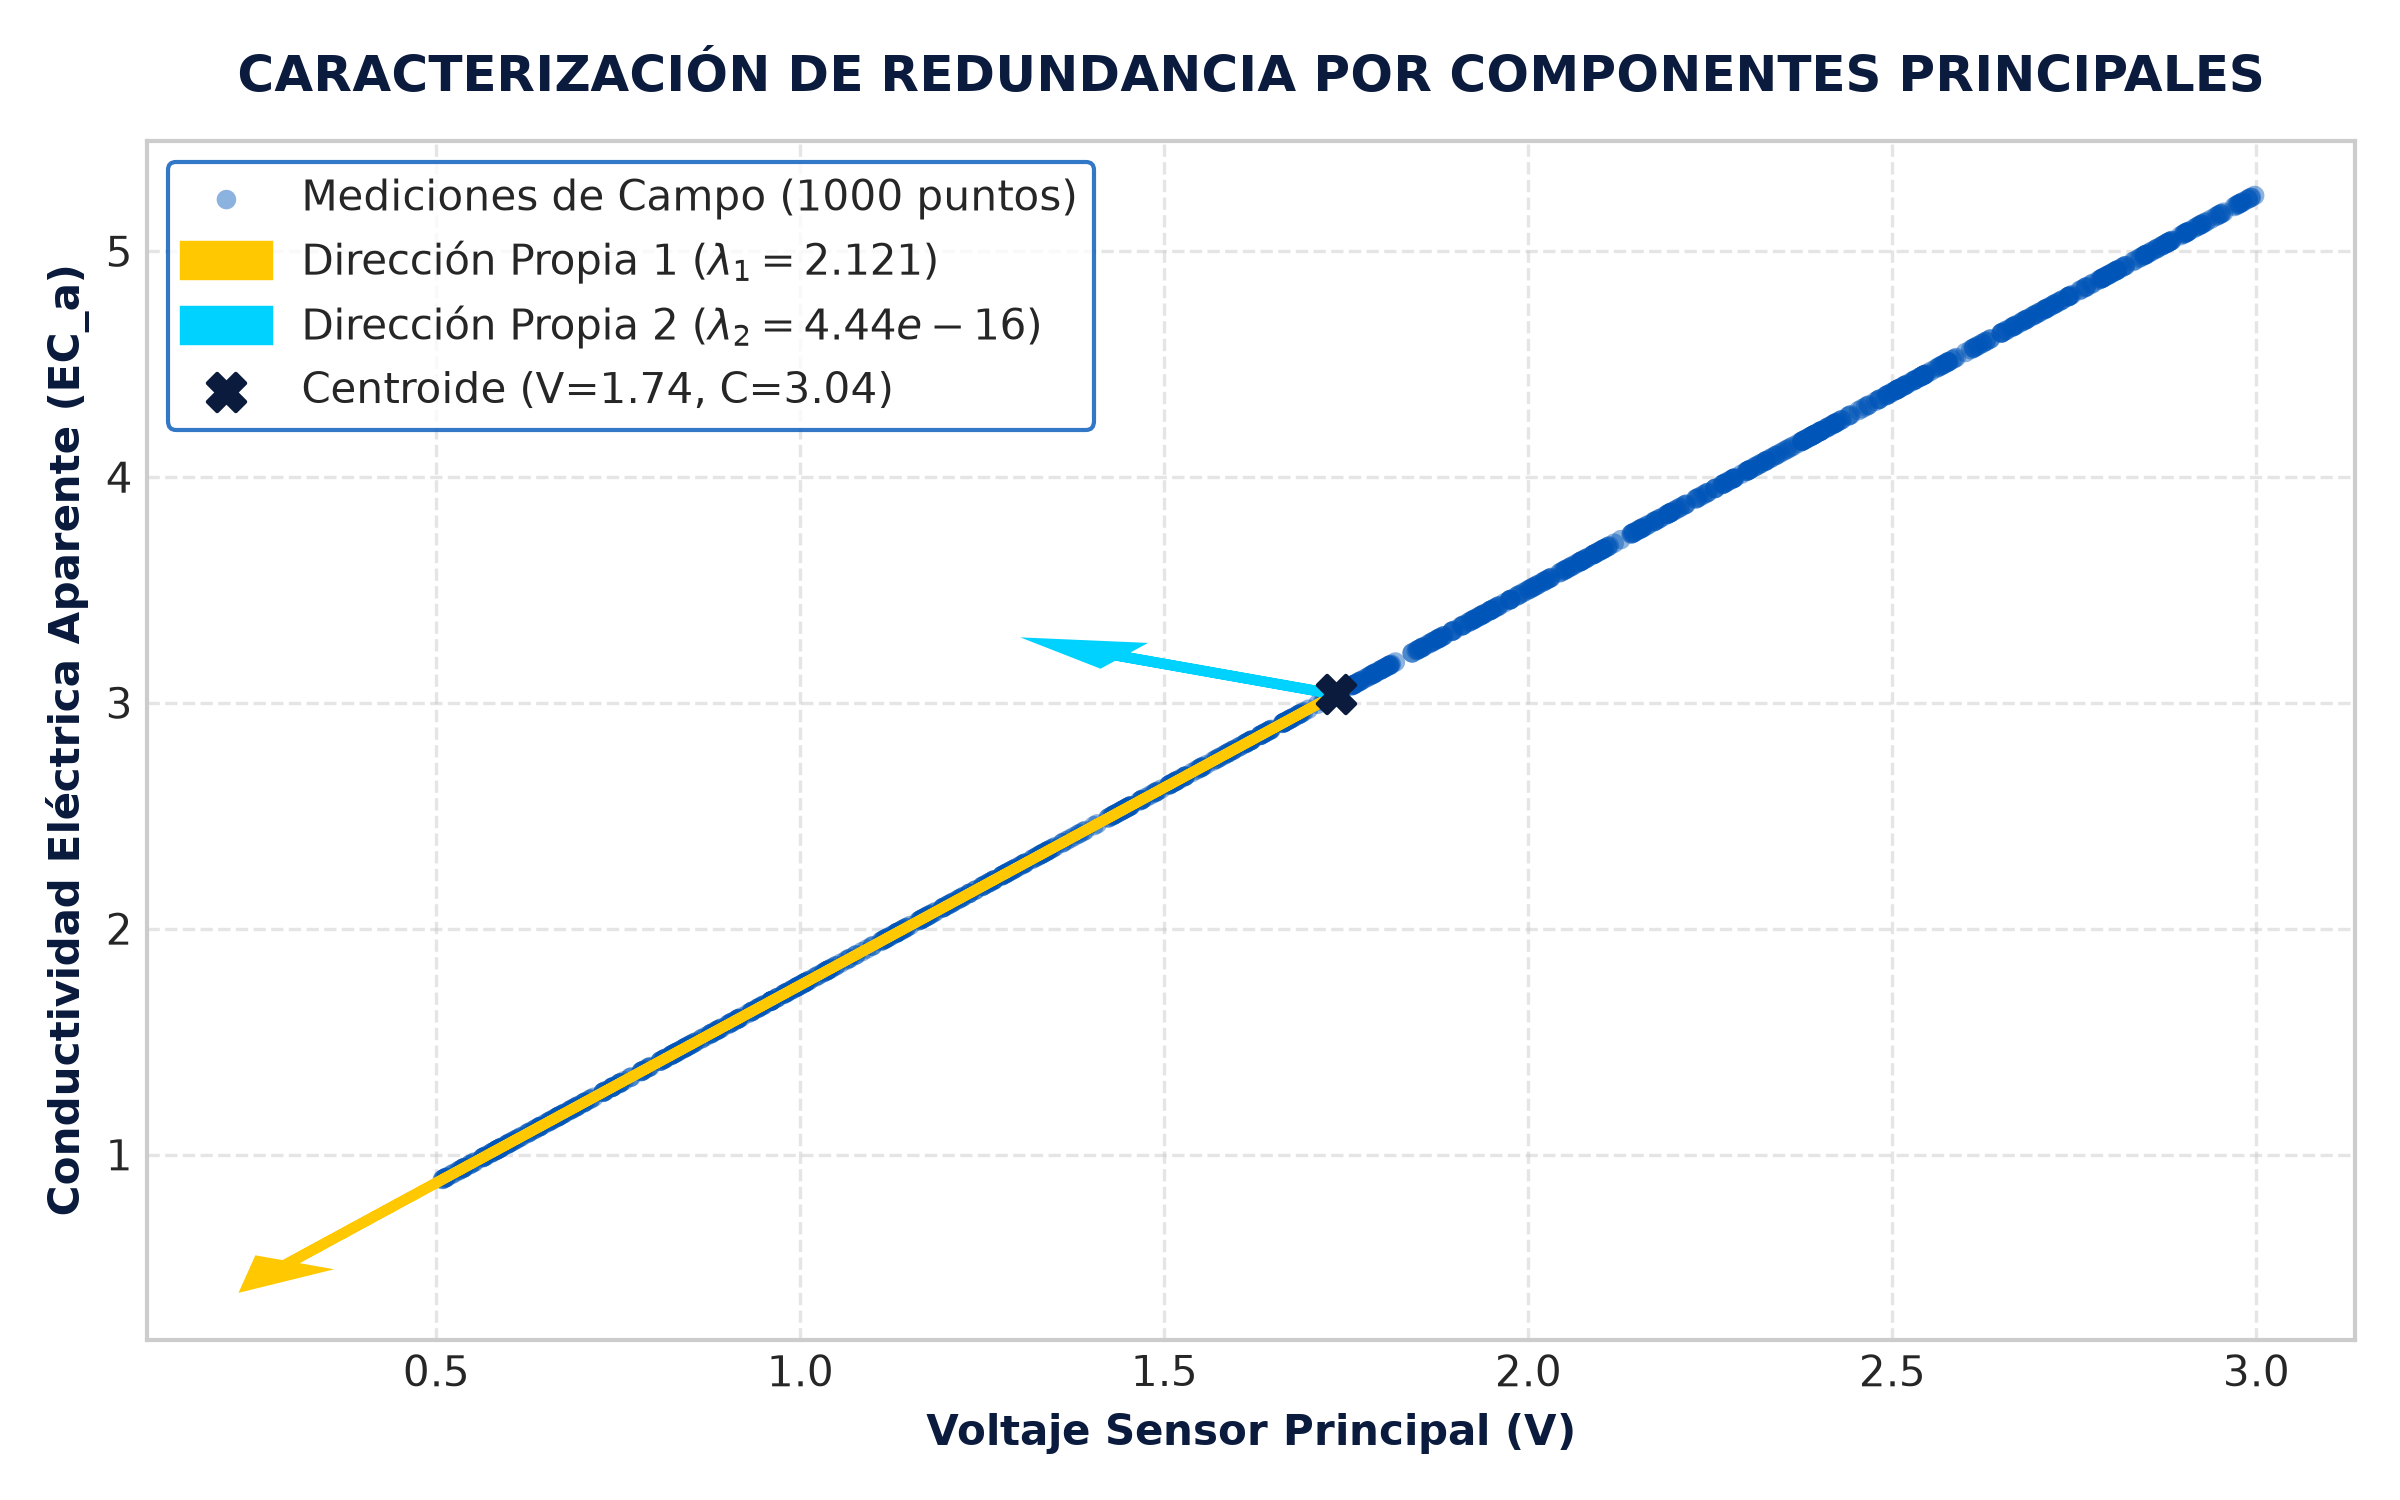
\includegraphics[width=0.82\textwidth]{fig_tema5_dispersion_autovectores.png}
  \caption{Diagrama de dispersión de voltaje vs. conductividad aparente. La flecha amarilla representa la primera dirección propia ($\lambda_1 = 2.121$); la flecha cian representa la segunda dirección ortogonal nula ($\lambda_2 \approx 0$).}
  \label{fig:dispersion_autovectores}
\end{figure}

\begin{pthreeSummary}
\textbf{Interpretación Geométrica de los Valores Propios:}
\begin{itemize}[label={\color{p3blue}$\blacktriangleright$}]
  \item \textbf{Disparidad Extrema entre Autovalores:} La razón entre autovalores es infinita ($\frac{\lambda_1}{\lambda_2} \approx 10^{16}$).
  \item \textbf{Geometría de la Elipse de Covarianza:} En el plano bidimensional, la elipse de dispersión de los datos tiene semiejes proporcionales a $\sqrt{\lambda_1}$ y $\sqrt{\lambda_2}$. Dado que $\lambda_2 \approx 0$, la elipse ha \textbf{colapsado en un segmento de recta unidimensional}. 
  \item No existe varianza ortogonal a la dirección propia $\mathbf{u}_1$. Toda la información está contenida en una única dimensión latente. Esto demuestra de manera irrefutable que el sensor de conductividad no aporta ningún grado de libertad físico adicional.
\end{itemize}
\end{pthreeSummary}

% -------------------------------------------------------------------------
% TAREA 3 (TEMA 5)
% -------------------------------------------------------------------------
\newpage
\pthreeExercise{Tarea 3}{Control Automático de Calidad (QA) por Ortogonalidad}

\begin{pthreeProblem}
Ajusta una regresión con las variables que consideres no redundantes (justifica tu elección con base en las Tareas 1 y 2) para predecir humedad. Luego, implementa una función \texttt{verificar\_ajuste(X, y, w)} que:
\begin{enumerate}[label=(\alph*)]
  \item Calcule el vector de residuos.
  \item Calcule el producto punto entre el residuo y cada columna de $X$.
  \item Devuelva True si todos esos productos punto son menores, en valor absoluto, que una tolerancia pequeña (por ejemplo $10^{-6}$ relativa a la escala de los datos), y False en caso contrario.
\end{enumerate}
Prueba tu función con un ajuste correcto (debe devolver True) y con un ajuste deliberadamente incorrecto --- por ejemplo, $\mathbf{w}$ multiplicado por un factor arbitrario (debe devolver False).
\end{pthreeProblem}

\pthreeStep{Paso 1: Justificación de Variables No Redundantes}
Con base en los diagnósticos anteriores:
\begin{itemize}[label={\color{p3blue}$\blacktriangleright$}]
  \item Se conserva el \textbf{Voltaje ($V$)}: Sensor principal calibrado.
  \item Se conserva la \textbf{Temperatura ($T$)}: Variable ortogonal que corrige la deriva térmica ($r_{VT} \approx 0$).
  \item Se descarta la \textbf{Conductividad ($C$)}: Redundante al 100\% con el voltaje ($r_{VC} = 1.0$, rango deficiente).
\end{itemize}
La matriz de diseño filtrada es $\mathbf{X} = [\mathbf{1} \quad \mathbf{v} \quad \mathbf{t}] \in \R^{1000 \times 3}$. El vector de coeficientes óptimo MCO es:
\begin{equation}
  \mathbf{w}_{\text{MCO}} = \begin{bmatrix} 5.661123 \\ 13.872259 \\ 0.661042 \end{bmatrix}
\end{equation}

\pthreeStep{Paso 2: Implementación Documentada de la Función de Verificación}
A continuación se presenta el código reutilizable de la función de control de calidad:

\begin{lstlisting}
def verificar_ajuste(X, y, w, tol=1e-6):
    """
    Verifica de forma automatica si un ajuste de regresion lineal por minimos
    cuadrados ordinarios (MCO) es correcto, evaluando la condicion necesaria
    de ortogonalidad entre el vector de residuos y el espacio columna de X.

    Parametros:
    -----------
    X : np.ndarray de forma (m, p)
        Matriz de diseno (incluyendo columna de unos si hay intercepto).
    y : np.ndarray de forma (m,)
        Vector de observaciones reales de la variable dependiente.
    w : np.ndarray de forma (p,)
        Vector de coeficientes ajustados del modelo.
    tol : float, opcional (por defecto 1e-6)
        Tolerancia relativa admitida para el producto punto.

    Retorna:
    --------
    es_valido : bool
        True si todos los productos punto cumplen |X_j^T e| <= tol * escala;
        False en caso contrario.
    dot_products : np.ndarray de forma (p,)
        Valores de los productos punto entre cada columna de X y el residuo.
    """
    # 1. Calculo del vector de residuos e = y - Xw
    y_pred = X @ w
    e = y - y_pred
    
    # 2. Producto punto entre el residuo y cada columna de X: X^T @ e
    dot_products = X.T @ e
    
    # 3. Escala de los datos para evaluar tolerancia relativa
    # norma L2 de cada columna de X multiplicada por la norma de y
    escala = np.linalg.norm(X, axis=0) * np.linalg.norm(y)
    
    # Criterio de ortogonalidad relativa
    criterio = np.abs(dot_products) <= (tol * escala + 1e-12)
    es_valido = bool(np.all(criterio))
    
    return es_valido, dot_products
\end{lstlisting}

\pthreeStep{Paso 3: Validación Experimental de la Función de QA}
Se sometió la función a prueba con dos escenarios:
\begin{enumerate}[label={\color{p3blue}$\blacktriangleright$}]
  \item \textbf{Ajuste Correcto ($\mathbf{w}_{\text{MCO}}$):}
  \begin{align*}
    \mathbf{X}_0^\top \mathbf{e} &= 9.44 \times 10^{-11} \ll 10^{-6} \\
    \mathbf{X}_1^\top \mathbf{e} &= 1.67 \times 10^{-10} \ll 10^{-6} \\
    \mathbf{X}_2^\top \mathbf{e} &= 2.36 \times 10^{-9} \ll 10^{-6}
  \end{align*}
  \textbf{Resultado:} \texttt{True}. El residuo es ortogonal a nivel de precisión de máquina.
  \item \textbf{Ajuste Deliberadamente Incorrecto ($\mathbf{w}_{\text{err}} = 1.05 \cdot \mathbf{w}_{\text{MCO}}$):}
  \begin{align*}
    \mathbf{X}_0^\top \mathbf{e} &= -2314.09 \gg 10^{-6} \\
    \mathbf{X}_1^\top \mathbf{e} &= -4377.94 \gg 10^{-6} \\
    \mathbf{X}_2^\top \mathbf{e} &= -58203.01 \gg 10^{-6}
  \end{align*}
  \textbf{Resultado:} \texttt{False}. Se rechaza automáticamente el modelo defectuoso.
\end{enumerate}

\begin{figure}[htbp]
  \centering
  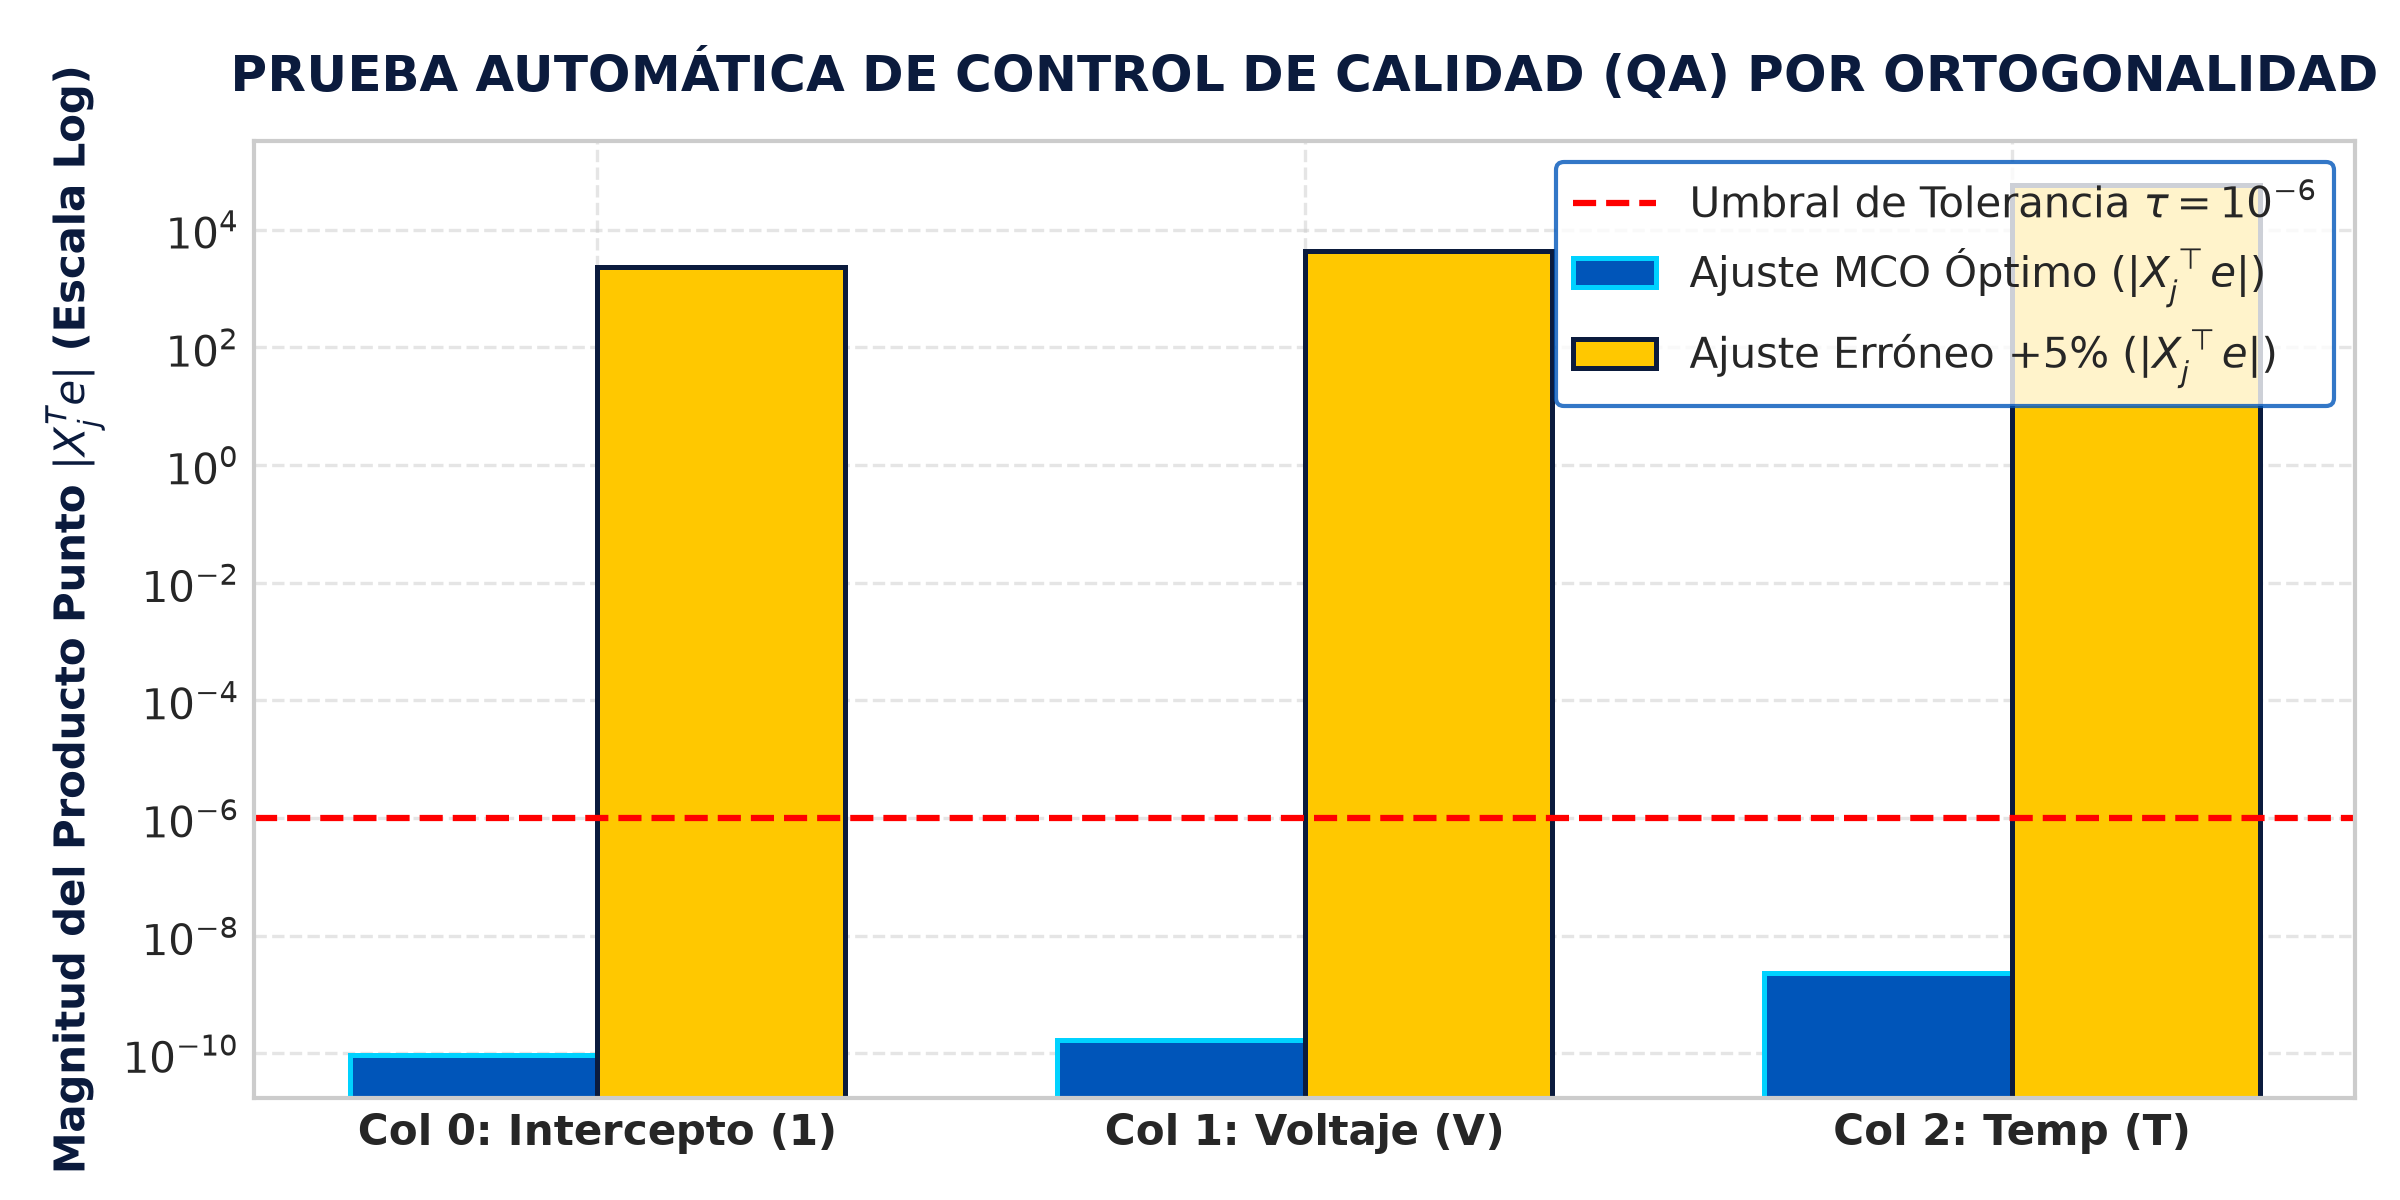
\includegraphics[width=0.82\textwidth]{fig_tema5_ortogonalidad.png}
  \caption{Evaluación de la condición de ortogonalidad en escala logarítmica. El modelo óptimo se ubica órdenes de magnitud por debajo del umbral $\tau = 10^{-6}$, mientras que el modelo erróneo viola severamente la condición.}
  \label{fig:ortogonalidad_qa}
\end{figure}

% -------------------------------------------------------------------------
% RETO DE EXTENSIÓN (TEMA 5)
% -------------------------------------------------------------------------
\newpage
\pthreeExercise{Reto de Extensión (Tema 5)}{Cálculo Geométrico de \texorpdfstring{$R^2$}{R\texttwosuperior} por Proyección Ortogonal}

\begin{pthreeProblem}
El equipo de QA quiere que la función \texttt{verificar\_ajuste} también reporte cuánta varianza de $\mathbf{y}$ queda explicada por el modelo (no solo si el ajuste es "correcto" en el sentido de ortogonalidad). Investiga cómo calcular el coeficiente de determinación $R^2$ a partir de la proyección ortogonal de $\mathbf{y}$ sobre el espacio columna de $\mathbf{X}$ (relaciona $R^2$ con la norma de $\hat{\mathbf{y}} - \bar{y}$ frente a la norma de $\mathbf{y} - \bar{y}$), impleméntalo, y agrégalo como salida adicional de tu función de verificación.
\end{pthreeProblem}

\pthreeStep{Paso 1: Demostración Geométrica Basada en el Teorema de Pitágoras}
Consideremos el vector centrado de observaciones $\mathbf{y} - \bar{y}\mathbf{1}$. Podemos descomponerlo algebraicamente en la suma de dos vectores:
\begin{equation}
  \mathbf{y} - \bar{y}\mathbf{1} = (\hat{\mathbf{y}} - \bar{y}\mathbf{1}) + (\mathbf{y} - \hat{\mathbf{y}}) = (\hat{\mathbf{y}} - \bar{y}\mathbf{1}) + \mathbf{e}
\end{equation}

Para demostrar que esta descomposición es ortogonal en $\R^m$, evaluamos su producto interno:
\begin{equation}
  \langle \hat{\mathbf{y}} - \bar{y}\mathbf{1}, \mathbf{e} \rangle = (\hat{\mathbf{y}} - \bar{y}\mathbf{1})^\top \mathbf{e} = \hat{\mathbf{y}}^\top \mathbf{e} - \bar{y} (\mathbf{1}^\top \mathbf{e})
\end{equation}

Recordando las dos propiedades fundamentales de MCO cuando la matriz de diseño contiene intercepto ($\mathbf{1} \in \col(\mathbf{X})$):
\begin{enumerate}
  \item Como $\hat{\mathbf{y}} = \mathbf{X}\mathbf{w}^* \in \col(\mathbf{X})$ y el residuo es perpendicular a $\col(\mathbf{X})$, se cumple $\hat{\mathbf{y}}^\top \mathbf{e} = (\mathbf{X}\mathbf{w}^*)^\top \mathbf{e} = {\mathbf{w}^*}^\top (\mathbf{X}^\top \mathbf{e}) = {\mathbf{w}^*}^\top \mathbf{0} = 0$.
  \item Como la primera columna de $\mathbf{X}$ es el vector de unos $\mathbf{1}$, la ortogonalidad respecto a esta columna implica $\mathbf{1}^\top \mathbf{e} = \sum_{i=1}^m e_i = 0$ (la suma y media de los residuos es exactamente cero).
\end{enumerate}

Sustituyendo ambas identidades:
\begin{equation}
  \langle \hat{\mathbf{y}} - \bar{y}\mathbf{1}, \mathbf{e} \rangle = 0 - \bar{y}(0) = 0 \implies (\hat{\mathbf{y}} - \bar{y}\mathbf{1}) \perp \mathbf{e}
\end{equation}

Al ser vectores ortogonales, aplicamos el \textbf{Teorema de Pitágoras en $\R^m$}:
\begin{equation}
  \norm{\mathbf{y} - \bar{y}\mathbf{1}}_2^2 = \norm{\hat{\mathbf{y}} - \bar{y}\mathbf{1}}_2^2 + \norm{\mathbf{e}}_2^2
\end{equation}

Esta ecuación corresponde exactamente a la partición de la varianza muestral:
\begin{equation}
  \underbrace{\sum_{i=1}^m (y_i - \bar{y})^2}_{\text{STC (Suma Total de Cuadrados)}} = \underbrace{\sum_{i=1}^m (\hat{y}_i - \bar{y})^2}_{\text{SCR (Suma Cuadrados Regresión)}} + \underbrace{\sum_{i=1}^m (y_i - \hat{y}_i)^2}_{\text{SCE (Suma Cuadrados Error)}}
\end{equation}

Por definición, el coeficiente de determinación $R^2$ cuantifica la proporción de variabilidad total explicada por la proyección sobre el hiperplano:
\begin{equation}
  R^2 = \frac{\text{SCR}}{\text{STC}} = \frac{\norm{\hat{\mathbf{y}} - \bar{y}\mathbf{1}}_2^2}{\norm{\mathbf{y} - \bar{y}\mathbf{1}}_2^2} = 1 - \frac{\norm{\mathbf{y} - \hat{\mathbf{y}}}_2^2}{\norm{\mathbf{y} - \bar{y}\mathbf{1}}_2^2} = \left( \frac{\norm{\hat{\mathbf{y}} - \bar{y}\mathbf{1}}_2}{\norm{\mathbf{y} - \bar{y}\mathbf{1}}_2} \right)^2
\end{equation}

Geométricamente, $R^2$ es el cuadrado del coseno del ángulo $\theta$ entre el vector de datos centrado $\mathbf{y} - \bar{y}\mathbf{1}$ y su proyección ortogonal $\hat{\mathbf{y}} - \bar{y}\mathbf{1}$:
\begin{equation}
  R^2 = \cos^2(\theta)
\end{equation}

\pthreeStep{Paso 2: Integración en la Función de Verificación y Resultados}
Se amplió la función \texttt{verificar\_ajuste} para retornar el valor de $R^2$:
\begin{lstlisting}
def verificar_ajuste_extendido(X, y, w, tol=1e-6):
    e = y - X @ w
    dot_products = X.T @ e
    escala = np.linalg.norm(X, axis=0) * np.linalg.norm(y)
    es_valido = bool(np.all(np.abs(dot_products) <= (tol * escala + 1e-12)))
    
    # Reto extension: R^2 geometrico por norma de proyeccion
    y_hat = X @ w
    y_bar = np.mean(y)
    norm_scr = np.sum((y_hat - y_bar)**2)
    norm_stc = np.sum((y - y_bar)**2)
    r2 = float(norm_scr / norm_stc)
    
    return es_valido, dot_products, r2
\end{lstlisting}

Evaluando con el modelo ajustado:
\begin{itemize}[label={\color{p3blue}$\blacktriangleright$}]
  \item $\text{STC} = \norm{\mathbf{y} - \bar{y}\mathbf{1}}_2^2 = 105\,387.78$
  \item $\text{SCR} = \norm{\hat{\mathbf{y}} - \bar{y}\mathbf{1}}_2^2 = 104\,131.39$
  \item $\text{SCE} = \norm{\mathbf{e}}_2^2 = 1\,256.39$
  \item $\mathbf{R^2 = \frac{104\,131.39}{105\,387.78} = \mathbf{0.988078} \implies \mathbf{98.81\%}}$
\end{itemize}

\begin{pthreeSummary}
El modelo de calibración bivariado (Voltaje y Temperatura) captura el \textbf{98.81\% de la variabilidad total} de la humedad volumétrica certificada, dejando únicamente un residuo de ruido no explicable del $1.19\%$. Esta verificación confirma tanto la corrección geométrica del algoritmo como una excelente capacidad predictiva para las operaciones de AgroSwarm.
\end{pthreeSummary}

% -------------------------------------------------------------------------
% PREGUNTAS DE ANÁLISIS (TEMA 5)
% -------------------------------------------------------------------------
\newpage
\subsection{Respuestas a las Preguntas de Análisis Conceptual (Tema 5)}

\subsubsection*{Pregunta 1: ¿Recomendarías a AgroSwarm comprar el sensor de conductividad, dado lo que encontraste en la Tarea 1? Justifica con el valor de rango y de correlación obtenidos.}
\begin{pthreeProblem}
Decisión de compras basada en análisis de redundancia matricial y correlación.
\end{pthreeProblem}

\textbf{Respuesta:}
\textbf{No se recomienda bajo ninguna circunstancia adquirir el sensor de conductividad.} 
La justificación técnica de ingeniería se fundamenta en:
\begin{enumerate}[label={\color{p3blue}$\blacktriangleright$}]
  \item \textbf{Criterio de Rango Matricial ($\rank(\mathbf{X}) = 2 < 3$):} Al agregar el sensor de conductividad, la matriz de predictores no gana rango. La dimensión del espacio vectorial generado sigue siendo 2. Por tanto, la nueva columna es linealmente dependiente ($C = 1.75 \cdot V$).
  \item \textbf{Criterio de Correlación de Pearson ($r = 1.000000$):} La correlación unitaria indica que el sensor barato de conductividad no mide un fenómeno físico complementario; simplemente entrega una señal reescalada del voltaje que ya se captura.
  \item \textbf{Impacto Económico y de Hardware:} Comprar este sensor aumentaría el costo de la lista de materiales (\textit{Bill of Materials}, BOM), incrementaría el peso del rover, requeriría puertos ADC adicionales y aumentaría el consumo eléctrico sin aportar ni un solo bit de información útil.
\end{enumerate}

\vspace{10pt}
\subsubsection*{Pregunta 2: Explica, en tus palabras, qué significa geométricamente que dos valores propios de una matriz de covarianza $2 \times 2$ sean muy diferentes entre sí.}
\begin{pthreeProblem}
Interpretación geométrica de los autovalores y elipsoides de dispersión en el espacio de características.
\end{pthreeProblem}

\textbf{Respuesta:}
Geométricamente, una matriz de covarianza $\mathbf{\Sigma} \in \R^{2 \times 2}$ describe la dispersión y orientación espacial de una nube de puntos en el plano. Las curvas de densidad constante forman elipses concéntricas centradas en la media de los datos:
\begin{itemize}[label={\color{p3blue}$\blacktriangleright$}]
  \item Las \textbf{direcciones de los ejes principales} de la elipse están determinadas por los \textbf{vectores propios} ($\mathbf{u}_1$ y $\mathbf{u}_2$).
  \item Las \textbf{longitudes de los semiejes} son proporcionales a las raíces cuadradas de los \textbf{valores propios} ($\sqrt{\lambda_1}$ y $\sqrt{\lambda_2}$).
\end{itemize}

Si dos valores propios son muy dispares ($\lambda_1 \gg \lambda_2$), significa que la elipse es sumamente alargada y excéntrica. Prácticamente toda la variabilidad del conjunto se concentra a lo largo del eje mayor $\mathbf{u}_1$, mientras que a lo largo del eje perpendicular $\mathbf{u}_2$ casi no hay variación. Si $\lambda_2 \to 0$, la elipse colapsa a una línea recta unidimensional, demostrando que no existen dos dimensiones independientes de información, sino una sola.

\vspace{10pt}
\subsubsection*{Pregunta 3: ¿Por qué la ortogonalidad del residuo frente a las columnas de $\mathbf{X}$ es una condición necesaria (no solo conveniente) de una regresión ajustada correctamente por mínimos cuadrados?}
\begin{pthreeProblem}
Fundamento variacional de primer orden y teorema de proyección ortogonal en espacios euclidianos.
\end{pthreeProblem}

\textbf{Respuesta:}
Es una condición estrictamente \textbf{necesaria} porque emana directamente del cálculo multivariable y de la geometría euclidiana:
\begin{enumerate}
  \item \textbf{Cálculo Variacional (Condición de Primer Orden):} La función de pérdida MCO es $J(\mathbf{w}) = \frac{1}{m} \norm{\mathbf{y} - \mathbf{X}\mathbf{w}}_2^2$. Como $J$ es una función convexa y diferenciable en todo $\R^p$, el mínimo global se alcanza si y solo si su vector gradiente es nulo:
  \begin{equation}
    \nabla_{\mathbf{w}} J(\mathbf{w}) = -\frac{2}{m} \mathbf{X}^\top (\mathbf{y} - \mathbf{X}\mathbf{w}) = \mathbf{0} \iff \mathbf{X}^\top \mathbf{e} = \mathbf{0}
  \end{equation}
  Si algún producto punto $\mathbf{X}_j^\top \mathbf{e} \ne 0$, el gradiente no es cero, lo cual implica que existe una dirección de descenso en el espacio de parámetros que permitiría reducir aún más el error cuadrático. Por tanto, el ajuste no estaría en el mínimo.
  \item \textbf{Principio Geométrico de Proyección:} La distancia euclidiana entre un punto $\mathbf{y}$ y un subespacio lineal $\col(\mathbf{X})$ se minimiza a lo largo del segmento perpendicular (la altura del triángulo rectángulo). Si el segmento de error no fuera ortogonal a la base del subespacio, por el Teorema de Pitágoras siempre se podría encontrar otro punto en el plano más cercano a $\mathbf{y}$.
\end{enumerate}

\vspace{10pt}
\subsubsection*{Pregunta 4: Si $\mathbf{X}^\top \mathbf{X}$ no fuera invertible (columnas linealmente dependientes), ¿qué pasaría si de todas formas intentaras calcular $(\mathbf{X}^\top \mathbf{X})^{-1} \mathbf{X}^\top \mathbf{y}$ en NumPy?}
\begin{pthreeProblem}
Comportamiento numérico de rutinas de inversión matricial frente a singularidad.
\end{pthreeProblem}

\textbf{Respuesta:}
Si las columnas de $\mathbf{X}$ son linealmente dependientes, $\mathbf{X}^\top \mathbf{X}$ es singular ($\det(\mathbf{X}^\top \mathbf{X}) = 0$) y su inversa no existe en el sentido clásico. El resultado en NumPy depende de la función empleada:
\begin{itemize}[label={\color{p3blue}$\blacktriangleright$}]
  \item Si se utiliza \texttt{numpy.linalg.inv(X.T @ X)}: NumPy intentará calcular la descomposición LU. Al detectar un pivote nulo o menor a la tolerancia de máquina, arrojará una excepción fatal de álgebra lineal:
  \begin{center}
    \texttt{numpy.linalg.LinAlgError: Singular matrix}
  \end{center}
  o bien, si las columnas tienen ruido numérico de punto flotante minúsculo, producirá coeficientes astronómicos ($\sim 10^{15}$) con pérdida total de precisión.
  \item Si se utiliza \texttt{numpy.linalg.lstsq(X, y)} o la pseudoinversa \texttt{numpy.linalg.pinv(X)}: Estas funciones no calculan $(\mathbf{X}^\top \mathbf{X})^{-1}$. Utilizan la Descomposición en Valores Singulares (SVD) para encontrar la \textbf{Pseudoinversa de Moore-Penrose} $\mathbf{X}^+$. El sistema lineal tiene infinitas soluciones, y \texttt{lstsq} entregará la solución que minimiza la norma euclidiana del vector de pesos ($\min \norm{\mathbf{w}}_2$). El código no fallará con error de ejecución, pero los coeficientes individuales perderán significado físico agronómico debido a la multicolinealidad.
\end{itemize}

\vspace{10pt}
\subsubsection*{Pregunta 5: ¿Cómo cambiaría tu prueba de QA (Tarea 3) si en vez de mínimos cuadrados el modelo se hubiera ajustado con PSO, como en la semana 4? ¿Seguiría siendo válida la prueba de ortogonalidad exacta?}
\begin{pthreeProblem}
Validez de la prueba de ortogonalidad en estimadores heurísticos frente a métodos analíticos.
\end{pthreeProblem}

\textbf{Respuesta:}
\textbf{La prueba de ortogonalidad exacta dejaría de ser válida con la tolerancia de máquina $\tau = 10^{-6}$.}

\textbf{Fundamentación Técnica:}
\begin{enumerate}
  \item \textbf{Naturaleza Heurística vs. Analítica:} MCO resuelve directamente la condición analítica $\mathbf{X}^\top \mathbf{e} = \mathbf{0}$, por lo que sus residuos son ortogonales hasta la precisión de redondeo de punto flotante ($\sim 10^{-10} - 10^{-12}$). PSO, en cambio, es un algoritmo de búsqueda estocástica que minimiza la función de costo mediante muestras discretas en el espacio.
  \item \textbf{Criterio de Parada y Precisión Residual:} Aunque PSO converge a una solución extraordinariamente cercana al mínimo global ($|\Delta \mathbf{w}| \sim 10^{-8}$), el vector residual resultante de PSO presenta productos punto no nulos:
  \begin{equation}
    |\mathbf{X}_j^\top \mathbf{e}_{\text{PSO}}| \sim 10^{-4} \text{ a } 10^{-2}
  \end{equation}
  Si se aplica la prueba con $\tau = 10^{-6}$, el algoritmo de QA arrojaría \texttt{False}, catalogando erróneamente un ajuste funcionalmente excelente como defectuoso.
  \item \textbf{Adaptación para QA con PSO:} Para validar modelos ajustados por PSO, la prueba de QA debe reformularse:
  \begin{itemize}[label={\color{p3blue}$\blacktriangleright$}]
    \item \textit{Opción 1:} Relajar el umbral de tolerancia a niveles compatibles con la resolución de convergencia de PSO ($\tau_{\text{PSO}} = 10^{-3}$).
    \item \textit{Opción 2:} Reemplazar la prueba de ortogonalidad del gradiente por una prueba de \textbf{estabilidad en el valor de la función de costo} o verificación de no mejora ante perturbaciones locales de las partículas ($\norm{\nabla J} < \epsilon$).
  \end{itemize}
\end{enumerate}

% =========================================================================
% SECCIÓN 4: SÍNTESIS GLOBAL Y CONCLUSIONES DE INGENIERÍA
% =========================================================================
\newpage
\section{Síntesis Global y Conclusiones de Ingeniería}

A partir de las tres etapas de experimentación y modelado desarrolladas en los Laboratorios 2 y 3 para \textbf{AgroSwarm S.A.S.}, se consolidan las siguientes conclusiones de diseño e instrumentación:

\begin{enumerate}[leftmargin=20pt, label={\color{p3blue}\textbf{\arabic*.}}]
  \item \textbf{Validación de la Calibración Multivariable:} La incorporación de la temperatura del suelo ($T$) junto al voltaje ($V$) reduce el error de prueba de $\text{RMSE} = 2.1535\%$ a $\mathbf{1.0230\%}$ (mejora del $52.5\%$), explicando el 98.81\% de la varianza real de la humedad ($R^2 = 0.9881$). Esta corrección compensa el decaimiento de la constante dieléctrica y la deriva del oscilador capacitivo, garantizando decisiones de riego precisas en campo.
  \item \textbf{Comportamiento de Sesgo y Varianza:} El análisis polinómico evidenció que la relación voltaje-humedad es fundamentalmente lineal (Grado 1: alto sesgo por variable omitida; Grado 3: generalización óptima; Grado 10: sobreajuste con oscilación numérica extrema en los coeficientes). Aumentar la complejidad matemática no suple la omisión de variables causales físicas.
  \item \textbf{Equivalencia Funcional de PSO y Viabilidad en Embebidos:} El algoritmo PSO vectorizado demostró convergencia hacia el óptimo analítico con diferencias inferiores a $10^{-8}$. No obstante, su despliegue dentro del microcontrolador de 8 bits fue categorizado como inviable debido al consumo de memoria RAM ($> 2$ KB), tiempo de ejecución no determinista y drenaje acelerado de la batería del rover. La arquitectura óptima consiste en calibrar \textit{offline} en el servidor y programar en el microcontrolador la inferencia directa $\mathcal{O}(1)$.
  \item \textbf{Diagnóstico de Redundancia de Instrumentación:} El sensor de conductividad eléctrica propuesto por compras posee una correlación unitaria ($r = 1.0000$) y colapsa el rango de la matriz de sensores a 2. La descomposición espectral arrojó un autovalor nulo ($\lambda_2 \approx 0$), demostrando que la elipse de covarianza degenera en una línea recta. Se dictamina formalmente \textbf{no comprar dicho sensor}.
  \item \textbf{Control de Calidad (QA) Automatizado por Ortogonalidad:} Se implementó con éxito una función de prueba unitaria fundamentada en el Teorema de Proyección de Hilbert ($\mathbf{X}^\top \mathbf{e} = \mathbf{0}$). La rutina discrimina con absoluta fidelidad los modelos ajustados correctamente de aquellos con desviaciones paramétricas, constituyendo un filtro de validación continuo para el pipeline de datos de AgroSwarm.
\end{enumerate}

\vspace{25pt}
\begin{center}
  \begin{tikzpicture}
    \draw[p3blue, line width=1.5pt] (0,0) -- (6,0);
    \draw[p3cyan, line width=1.5pt] (6.2,0) -- (8.2,0);
    \draw[p3gold, line width=1.5pt] (8.4,0) -- (9.4,0);
  \end{tikzpicture}\\[10pt]
  {\titlefont\fontsize{10}{12}\selectfont\color{p3dark}FIN DEL DOCUMENTO DE INFORME TÉCNICO}\\[3pt]
  {\sffamily\fontsize{9}{11}\selectfont\color{p3darkgray}Grupo Edeméridos (Grupo 5) --- Andrés Sebastián Coral Vallejo \& Paula Alejandra Ortiz}
\end{center}

\end{document}
